%% Author: Leighton Pritchard
%% Copyright: James Hutton Institute
%% 2016-03-21: Slides for teaching at University of Dundee, 21st March 2016
%% This presentation was an invited lecture on comparative genomics and visualisation
%% for the BS32010 course.

%% UNCOMMENT FOR SLIDES
\documentclass[table]{beamer}
\mode<presentation>

%% UNCOMMENT FOR HANDOUTS
%\documentclass[handout]{beamer}
\usepackage{handoutWithNotes}
\pgfpagesuselayout{4 on 1 with notes}[a4paper,border shrink=5mm]

%% GENERIC STYLE SETTINGS BELOW
\usetheme{default}
\usepackage{listings}
\usepackage{multirow}
\usepackage{xcolor}
\usepackage{hyperref}
%\usepackage[multiple]{footmisc}

\usebackgroundtemplate{

\includegraphics[width=\paperwidth,height=\paperheight]{images/hutton_background}
}
%% PRESENTATION CONFIGURATION PARAMETERS %%%%%%%%%%%%%%%%%%%%%%%%%%%%%%%%%%%%%%%
%\titlebackgroundfile{images/hutton_title}
%\framebackgroundfile{images/hutton_background}
\definecolor{hutton_green}{HTML}{78A22F}
\definecolor{hutton_purple}{HTML}{872175}
\definecolor{hutton_blue}{HTML}{569BBE}
\definecolor{olive}{rgb}{0.3, 0.4, .1}
\definecolor{fore}{RGB}{249,242,215}
\definecolor{back}{RGB}{51,51,51}
\definecolor{title}{RGB}{255,0,90}
\definecolor{dgreen}{rgb}{0.,0.6,0.}
\definecolor{gold}{rgb}{1.,0.84,0.}
\definecolor{JungleGreen}{cmyk}{0.99,0,0.52,0}
\definecolor{BlueGreen}{cmyk}{0.85,0,0.33,0}
\definecolor{RawSienna}{cmyk}{0,0.72,1,0.45}
\definecolor{Magenta}{cmyk}{0,1,0,0}
\usefonttheme{structurebold}
\setbeamercolor{alerted text}{fg=orange}
\setbeamercolor{background canvas}{bg=white}
\setbeamercolor{block title}{bg=hutton_purple}
\setbeamercolor{frametitle}{fg=hutton_purple}
\setbeamercolor{title}{fg=black}
\setbeamercolor{titlelike}{fg=hutton_green}
\setbeamercolor{author}{fg=hutton_purple}
\setbeamercolor{author in head/foot}{fg=white}
\setbeamercolor{title in head/foot}{fg=white}
\setbeamercolor{section in head/foot}{fg=hutton_purple}
\setbeamercolor{normal text}{fg=black}
\setbeamercolor{frametitle}{fg=hutton_purple}
\setbeamerfont{block title}{size={}}
\setbeamerfont{author}{size=\footnotesize}
\setbeamerfont{institute}{size=\tiny}
\setbeamerfont{date}{size=\footnotesize}
\setbeamercolor{section in toc shaded}{fg=hutton_purple}
\setbeamercolor{section in toc}{fg=hutton_purple}
\setbeamercolor{subsection in toc shaded}{fg=hutton_purple}
\setbeamercolor{subsection in toc}{fg=hutton_purple}
\setbeamertemplate{itemize item}[circle]
\setbeamertemplate{itemize subitem}[circle]
\setbeamertemplate{itemize subsubitem}[circle]
\setbeamertemplate{itemize subsubsubitem}[circle]
\setbeamercolor{itemize item}{fg=hutton_purple}
\setbeamercolor{itemize subitem}{fg=hutton_purple}
\setbeamercolor{itemize subsubitem}{fg=hutton_purple}
\setbeamercolor{itemize subsubsubitem}{fg=hutton_purple}
\setbeamercolor{enumerate item}{fg=hutton_purple}
\setbeamercolor{enumerate subitem}{fg=hutton_purple}
\setbeamercolor{enumerate subsubitem}{fg=hutton_purple}
\setbeamercolor{enumerate subsubsubitem}{fg=hutton_purple}
\setbeamercolor{alerted text}{fg=hutton_green}
\setbeamerfont{alerted text}{series=\bfseries}
% This command makes sure that acrobat reader doesn't change the colours of the slide
% when there are figures with transparencies.
\pdfpageattr {/Group << /S /Transparency /I true /CS /DeviceRGB>>}

%Disables discrete bottom navigation bar
\beamertemplatenavigationsymbolsempty

% Modify the slide titles to avoid the corner images,
\setbeamertemplate{frametitle}
{
\vspace{0.05\textheight}
\noindent\quad\begin{minipage}[t][0.12\textheight][t]{0.85\textwidth}
\insertframetitle\par
\end{minipage}
}

% Modify title page to avoid the big logo on right
\setbeamertemplate{title page}{
    \begin{picture}(0,0)
            %This ends up on top of the default background image, rather than replacing it:
            \put(-30,-165){%
                
\includegraphics[width=\paperwidth,height=\paperheight]{images/hutton_title}
            }
            \put(0,-75){%
                \begin{minipage}[b][0.4\textheight][t]{0.75\textwidth}
                    \usebeamerfont{title}\usebeamercolor[fg]{title}{\inserttitle\par}
                    \usebeamerfont{subtitle}\usebeamercolor[fg]{subtitle}{\insertsubtitle\par}
                \end{minipage}
            }
            \put(0,-125){%
                \begin{minipage}[b][0.1\textheight][t]{\textwidth}
                    \usebeamerfont{author}\usebeamercolor[fg]{author}{\insertauthor\par}
                    \usebeamerfont{institute}\usebeamercolor[fg]{institute}{\insertinstitute\par}
                \end{minipage}
            }
    \end{picture}
}

% Make \verbatim environment tiny font
\makeatletter
\def\verbatim{\tiny\@verbatim \frenchspacing\@vobeyspaces \@xverbatim}
\makeatother

%%%%%%%%%%%%%%%%%%%%%%%%%%%%%%%%%%%%%%%%%%%%%%%%%%%%%%%%%%%%%%%%%%%%%%%%%%%%%%%%

% LISTINGS SETTING
% Settings for code listings in lstlistings

\definecolor{hutton_lightgreen}{HTML}{C8F27F}

\lstset{ %
  backgroundcolor=\color{hutton_lightgreen},   % choose the background color; you must add \usepackage{color} or \usepackage{xcolor}
  basicstyle=\tiny\ttfamily,        % the size of the fonts that are used for the code
  breakatwhitespace=false,         % sets if automatic breaks should only happen at whitespace
  breaklines=true,                 % sets automatic line breaking
  captionpos=b,                    % sets the caption-position to bottom
  commentstyle=\color{red},    % comment style
  deletekeywords={...},            % if you want to delete keywords from the given language
  escapeinside={\%*}{*)},          % if you want to add LaTeX within your code
  extendedchars=true,              % lets you use non-ASCII characters; for 8-bits encodings only, does not work with UTF-8
  frame=single,                    % adds a frame around the code
  keepspaces=true,                 % keeps spaces in text, useful for keeping indentation of code (possibly needs columns=flexible)
  keywordstyle=\color{blue},       % keyword style
%  language=Octave,                 % the language of the code
  morekeywords={*,...},            % if you want to add more keywords to the set
  numbers=left,                    % where to put the line-numbers; possible values are (none, left, right)
  numbersep=5pt,                   % how far the line-numbers are from the code
  numberstyle=\tiny\color{gray}, % the style that is used for the line-numbers
  rulecolor=\color{black},         % if not set, the frame-color may be changed on line-breaks within not-black text (e.g. comments (green here))
  showspaces=false,                % show spaces everywhere adding particular underscores; it overrides 'showstringspaces'
  showstringspaces=false,          % underline spaces within strings only
  showtabs=false,                  % show tabs within strings adding particular underscores
  stepnumber=1,                    % the step between two line-numbers. If it's 1, each line will be numbered
  stringstyle=\color{violet},     % string literal style
  tabsize=4,                       % sets default tabsize to 2 spaces
  title=\lstname                   % show the filename of files included with \lstinputlisting; also try caption instead of title
}


%%%
% TITLE PREAMBLE
\title[Comparative Genomics and Visualisation] % (optional, only for long titles)
{Comparative Genomics and \\ Visualisation \\
BS32010 \\}
%\subtitle{}
\author[Pritchard] % (optional, for multiple authors)
{Leighton~Pritchard$^{1,2,3}$}
\institute[The James Hutton Institute] % (optional)
{
  $^{1}$Information and Computational Sciences,\\
  $^{2}$Centre for Human and Animal Pathogens in the Environment,\\
  $^{3}$Dundee Effector Consortium,\\
  The James Hutton Institute, Invergowrie, Dundee, Scotland, DD2 5DA
}
\date[21st March 2016] % (optional)
{21st March 2016}
\subject{Bioinformatics, Genomics, Bacteria, Sequencing, Microbiology, Microbes, Comparative Genomics, Visualisation}

%%%
% TOC
% Show table of contents, with current section highlighted,
% at the start of each section

%\AtBeginSection[]
%{
%  \begin{frame}
%    \frametitle{Table of Contents}
%    \tableofcontents[currentsection] %,hideallsubsections]
%  \end{frame}
%}

\AtBeginSubsection[]
{
  \begin{frame}
    \frametitle{Table of Contents}
    \tableofcontents[currentsection,currentsubsection] %,hideallsubsections]
  \end{frame}
}

%%%
% START DOCUMENT
\begin{document}

\frame[plain]{\titlepage}

%% use.tex
%% Author: Leighton Pritchard
%% Copyright: James Hutton Institute
%% These slides describe the acceptable use policy for these slides and
%% materials

%
\begin{frame}
  \frametitle{Acceptable Use Policy}
  Recording of this talk, taking photos, discussing the content using \\
  email, Twitter, blogs, etc. is permitted (and encouraged), \\
  providing distraction to others is minimised. \\[0.5cm]
  These slides will be made available on SlideShare. \\[0.5cm]
  \textbf{These slides, and supporting material including exercises, are available at \href{https://github.com/widdowquinn/Teaching-2015-03-17-UoD_compgenvis}{https://github.com/widdowquinn/Teaching-2015-03-17-UoD\_compgenvis}}
\end{frame}

%%%
% SECTION: Introduction
\section{Introduction}

%% SUBSECTION
%% What is Comparative Genomics?
\subsection{What is comparative genomics?}
%% what_is_compgen.tex
%% Author: Leighton Pritchard
%% Copyright: James Hutton Institute
%% Introductory slides: What is Comparative Genomics?





%
\begin{frame}
  \frametitle{What Is Comparative Genomics?}
  \Large{
    \textcolor{olive}{
      \textbf{
      The combination of genomic data, and comparative and evolutionary biology, to address questions of   genome structure, evolution, and function.
      }
    }
  }
\end{frame}

%
\begin{frame}
  \frametitle{Evolution is the central concept}
  \begin{center}
    
\includegraphics[width=\textwidth]{images/dobzhansky_quote}
  \end{center}  
\end{frame}

%
\begin{frame}
  \frametitle{Comparison of physical features}
  How do we determine that features are related, and evolved? \\
  \begin{center}
    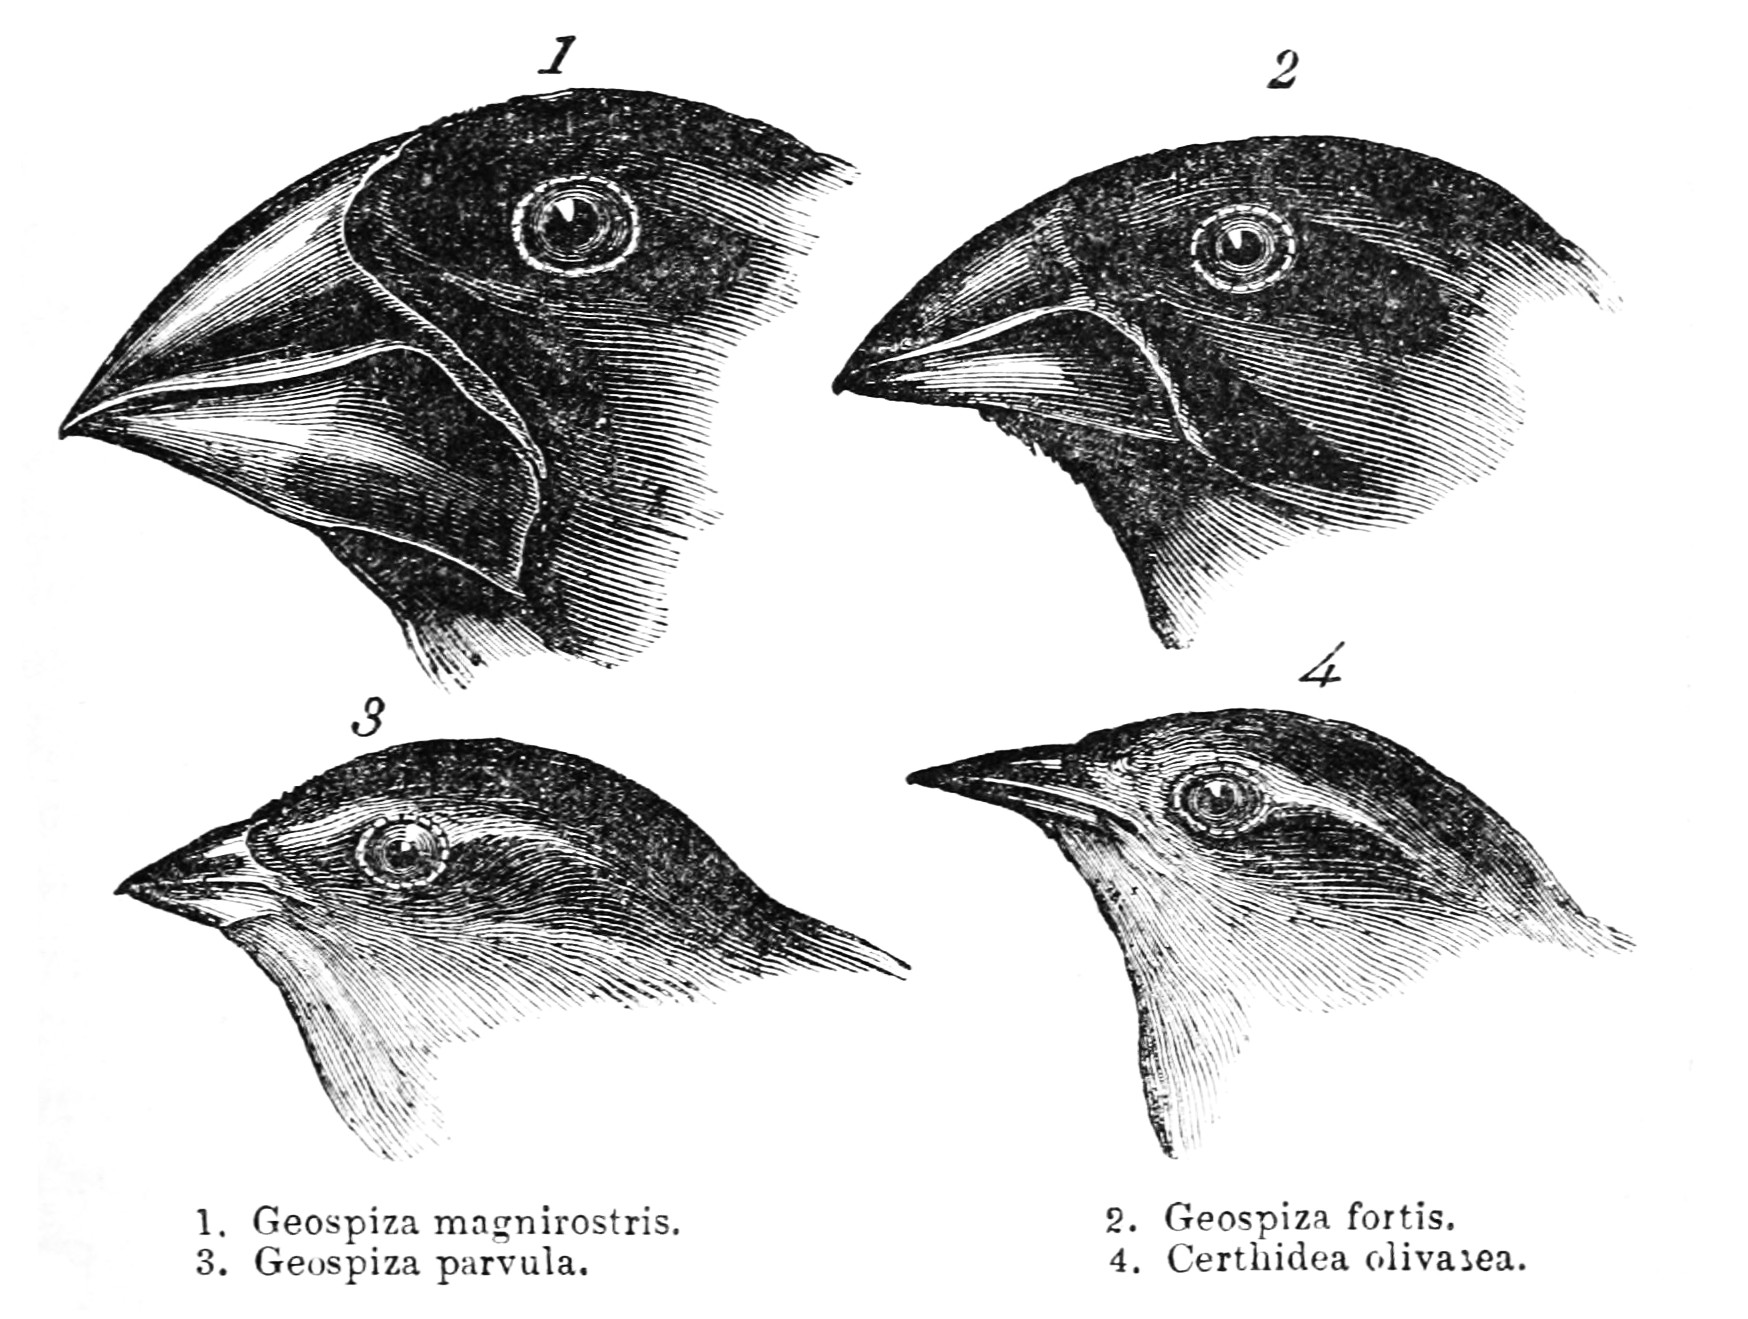
\includegraphics[width=0.8\textwidth]{images/darwin_finches}
  \end{center}  
\end{frame}

%
\begin{frame}
  \frametitle{Comparison of sequence features}
  Multiple sequence alignment of ATP synthase \\
  \begin{center}
    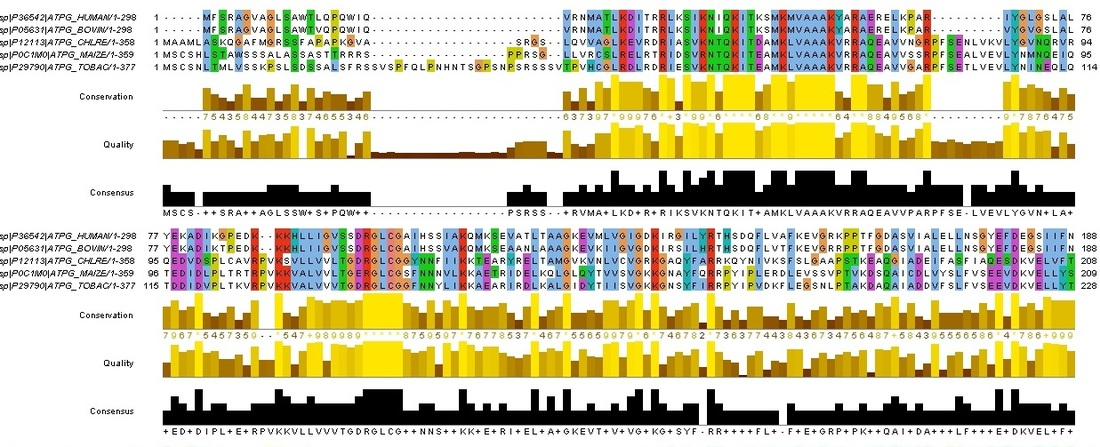
\includegraphics[width=\textwidth]{images/atp_synthase_alignment}
  \end{center}  
\end{frame}

%
\begin{frame}
  \frametitle{Comparison of genome features}
  Similarity of individual features (feature sequence) \\
  \begin{center}
    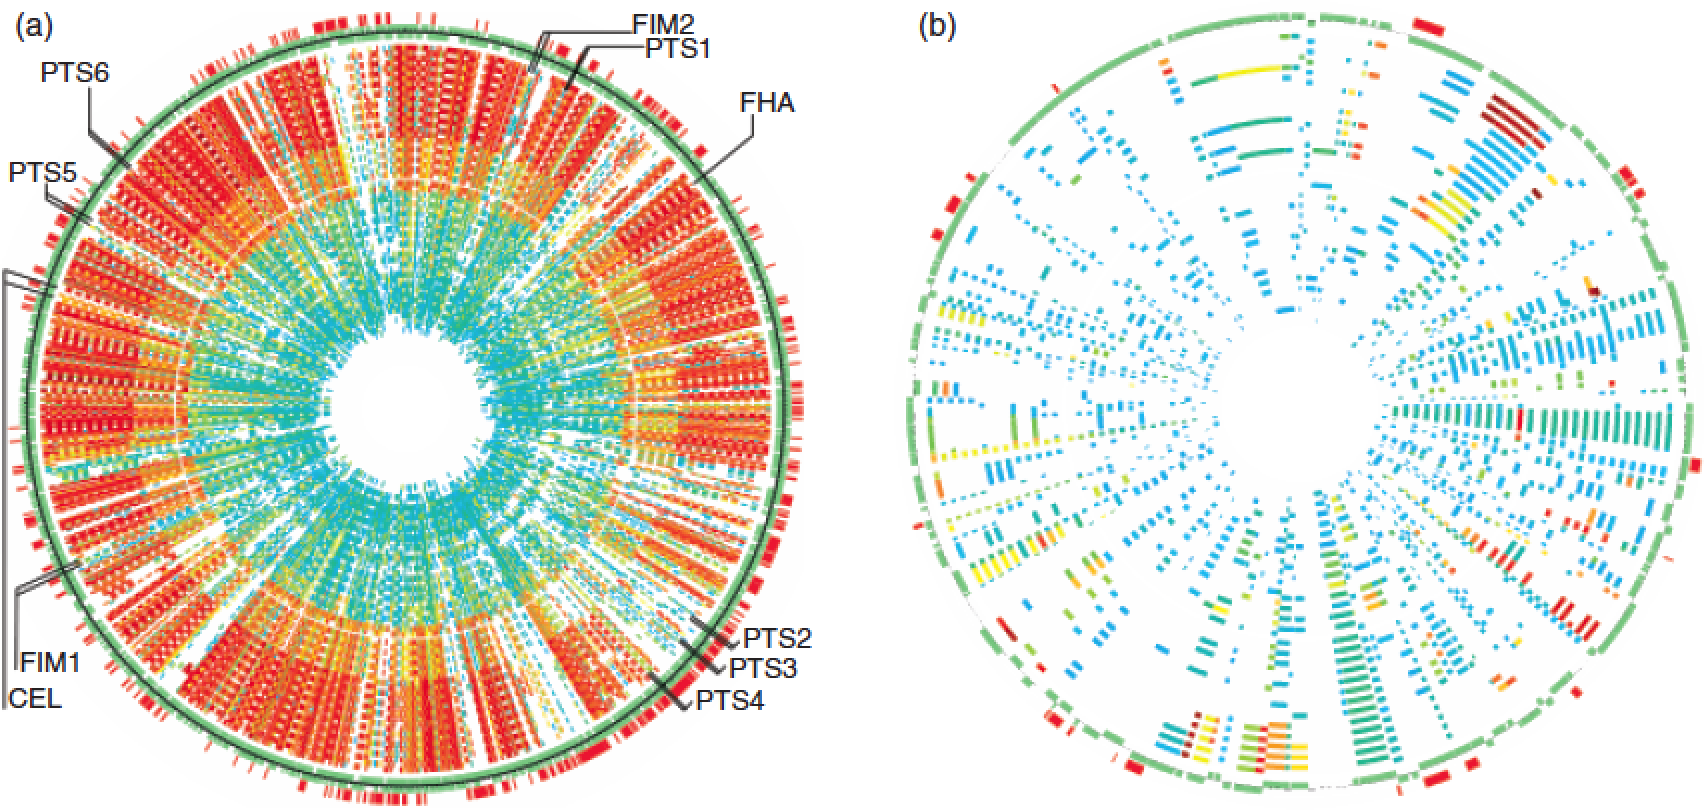
\includegraphics[width=\textwidth]{images/salmonella_circular_comparison}
  \end{center}  
\end{frame}

%
\begin{frame}
  \frametitle{Comparison of genome features}
  Similarity of individual features (ordering and arrangement) \\
  \begin{center}
    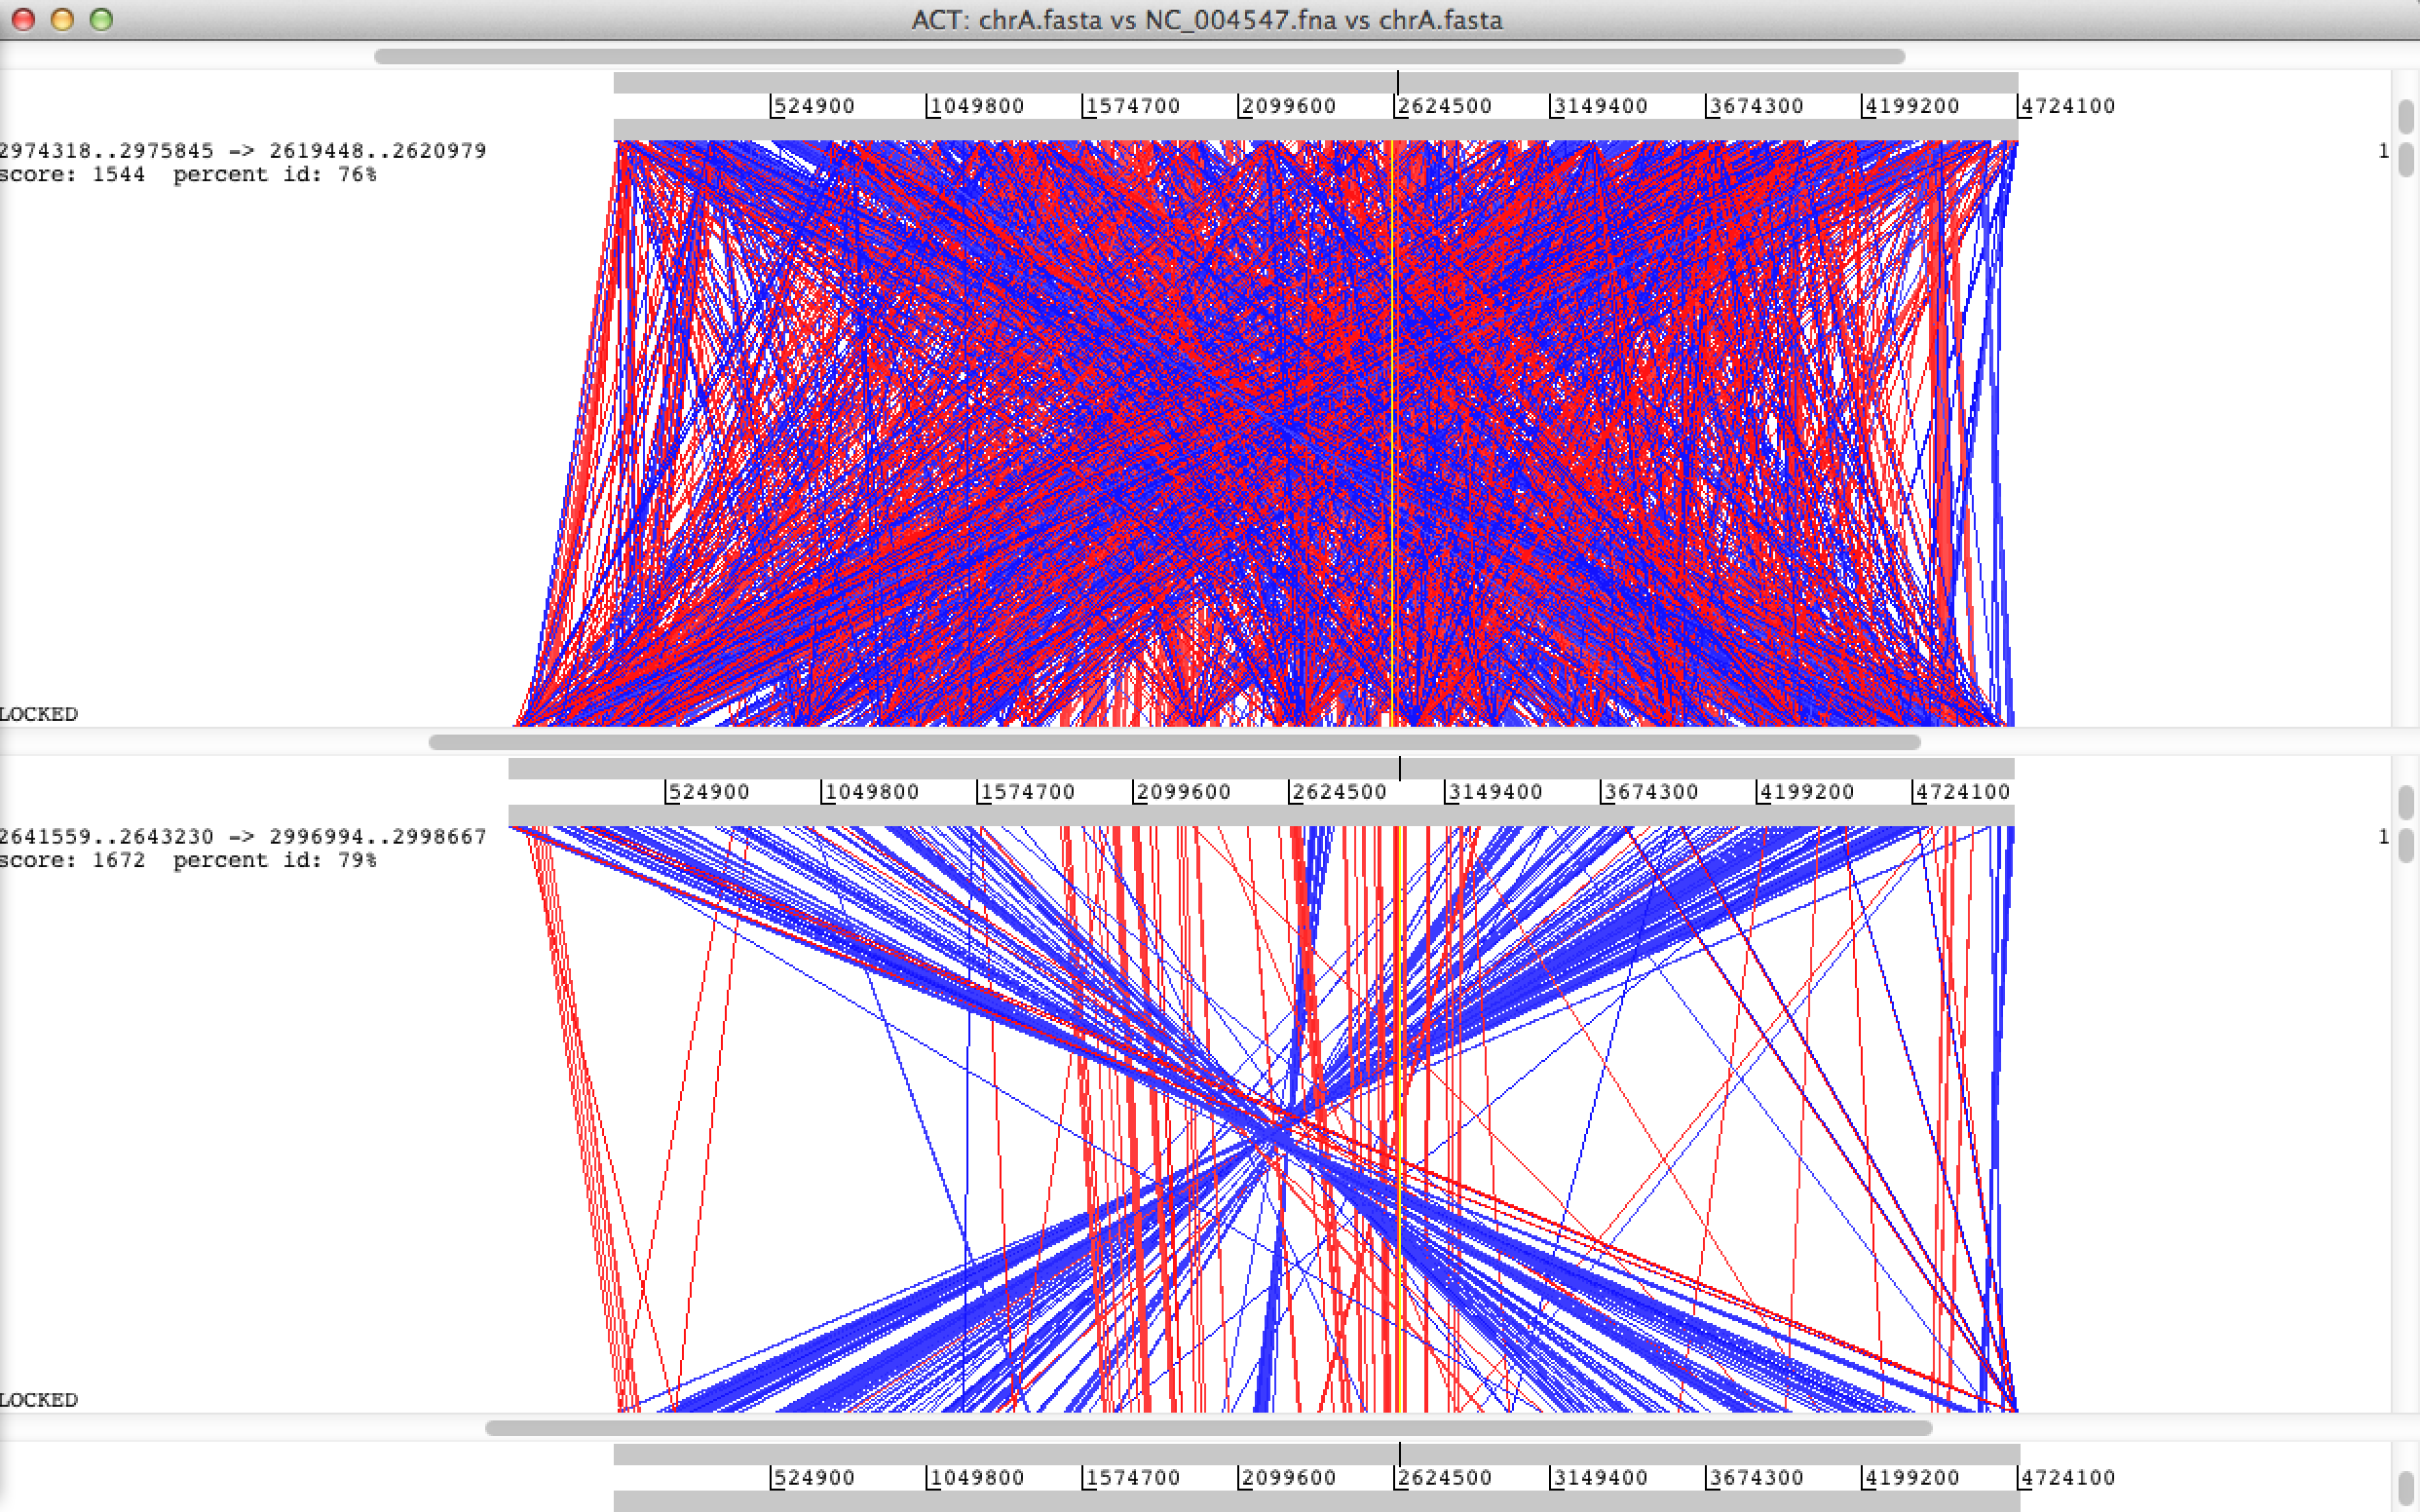
\includegraphics[width=\textwidth]{images/act_rearrangement}
  \end{center}  
\end{frame}

%
\begin{frame}
  \frametitle{Why comparative genomics?}
    \begin{columns}[c] 
      \column{.6\textwidth} 
        \begin{itemize}
         \item \textcolor{hutton_green}{Genome features are heritable characteristics}
         \item \textcolor{hutton_purple}{Related organisms share ancestral genomes}
         \item \textcolor{hutton_blue}{Related organisms inherit common genome features}
         \item \textcolor{RawSienna}{Genome similarity $\propto$ relatedness? (phylogenomics)}
        \end{itemize}
      \column{.4\textwidth}
        
\includegraphics[width=\textwidth]{images/darwin_tree}
    \end{columns}  
\end{frame}

%
\begin{frame}
  \frametitle{Why comparative genomics?}
    \begin{columns}[c] 
      \column{.6\textwidth} 
        \begin{itemize}
         \item \textcolor{hutton_green}{Genomes carry functional elements under selection pressure}
         \item \textcolor{hutton_purple}{Related organisms carry similar functional elements}
         \item \textcolor{hutton_blue}{Deleterious functional elements are lost through selection}         
         \item \textcolor{RawSienna}{Genome similarity $\propto$ phenotype? (functional genomics)}         
        \end{itemize}
      \column{.4\textwidth}
        
\includegraphics[width=\textwidth]{images/darwin_tree}
    \end{columns}  
\end{frame}

%
\begin{frame}
  \frametitle{Why comparative genomics?}
    \begin{columns}[c] 
      \column{.6\textwidth} 
        \begin{itemize}
         \item \textcolor{hutton_green}{Functional elements are selected over many generations}
         \item \textcolor{hutton_purple}{Optimised functional elements may not change greatly}
         \item \textcolor{hutton_blue}{(Functional elements can be transferred non-heritably)}   
         \item \textcolor{RawSienna}{Genome feature similarity $\implies$ common function? (genome annotation)}
         \item \textcolor{red}{Transfer functional information from model systems (\textit{E. coli}, \textit{A. thaliana}, \textit{D. melanogaster}) to non-model systems}
        \end{itemize}
      \column{.4\textwidth}
        
\includegraphics[width=\textwidth]{images/darwin_tree}
    \end{columns}  
\end{frame}

%
\begin{frame}
  \frametitle{Genomes are informative, but$\ldots$}
  \textcolor{hutton_blue}{\textbf{BIOLOGICAL CONTEXT:}} epigenetics, tissue differentiation, mesoscale systems, etc.\\
  \begin{center}  
    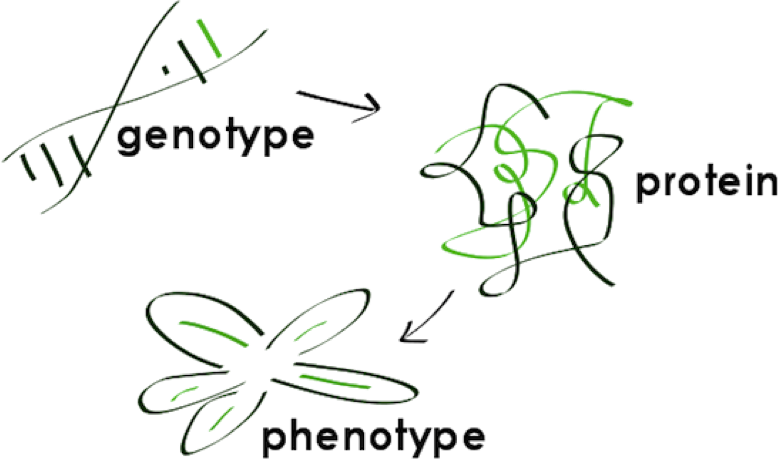
\includegraphics[width=0.7\textwidth]{images/genotype_protein_phenotype}
  \end{center}    
  \textcolor{hutton_green}{\textbf{PHENOTYPIC PLASTICITY:}} responses to temperature, stress, environment, etc.
\end{frame}

%
\begin{frame}
  \frametitle{Genomes to systems}
    \begin{columns}[c] 
      \column{.6\textwidth} 
        \textcolor{RawSienna}{\textbf{Functional Genomics}}
        \begin{itemize}
         \item \textcolor{hutton_green}{Genome differences underpin phenotype (morphological, physiological) differences.}
         \item \textcolor{hutton_purple}{If phenotypes known, genome comparisons can indicate genomic origin of differences (e.g. GWAS).}
         \item \textcolor{hutton_blue}{Genome comparisons can reveal evolutionary processes and constraints, and suggest phenotypic outcomes.}
        \end{itemize}
      \column{.4\textwidth}
        
\includegraphics[width=\textwidth]{images/darwin_tree}
    \end{columns}  
\end{frame}




%% SUBSECTION
%% Levels of genome comparison (species, genus, etc.)
\subsection{Levels of genome comparison}
%% cladograms.tex
%% Author: Leighton Pritchard
%% Copyright: James Hutton Institute
%% Introductory slides: Cladograms.

%
\begin{frame}
  \frametitle{Types of comparison}
    \begin{columns}[T] 
      \column{.5\textwidth} 
        \textcolor{RawSienna}{\textbf{Within species}}
        \begin{itemize}
	  \item e.g. between isolates/individuals (or between tissues$\ldots$)
	  \item \textcolor{hutton_green}{Which genome features may account for unique characteristics of organisms or cell-types (e.g. tumours)?}
	  \item \textcolor{hutton_blue}{what epigenetic changes occur in an individual?}
	\end{itemize}
      \column{.5\textwidth}
        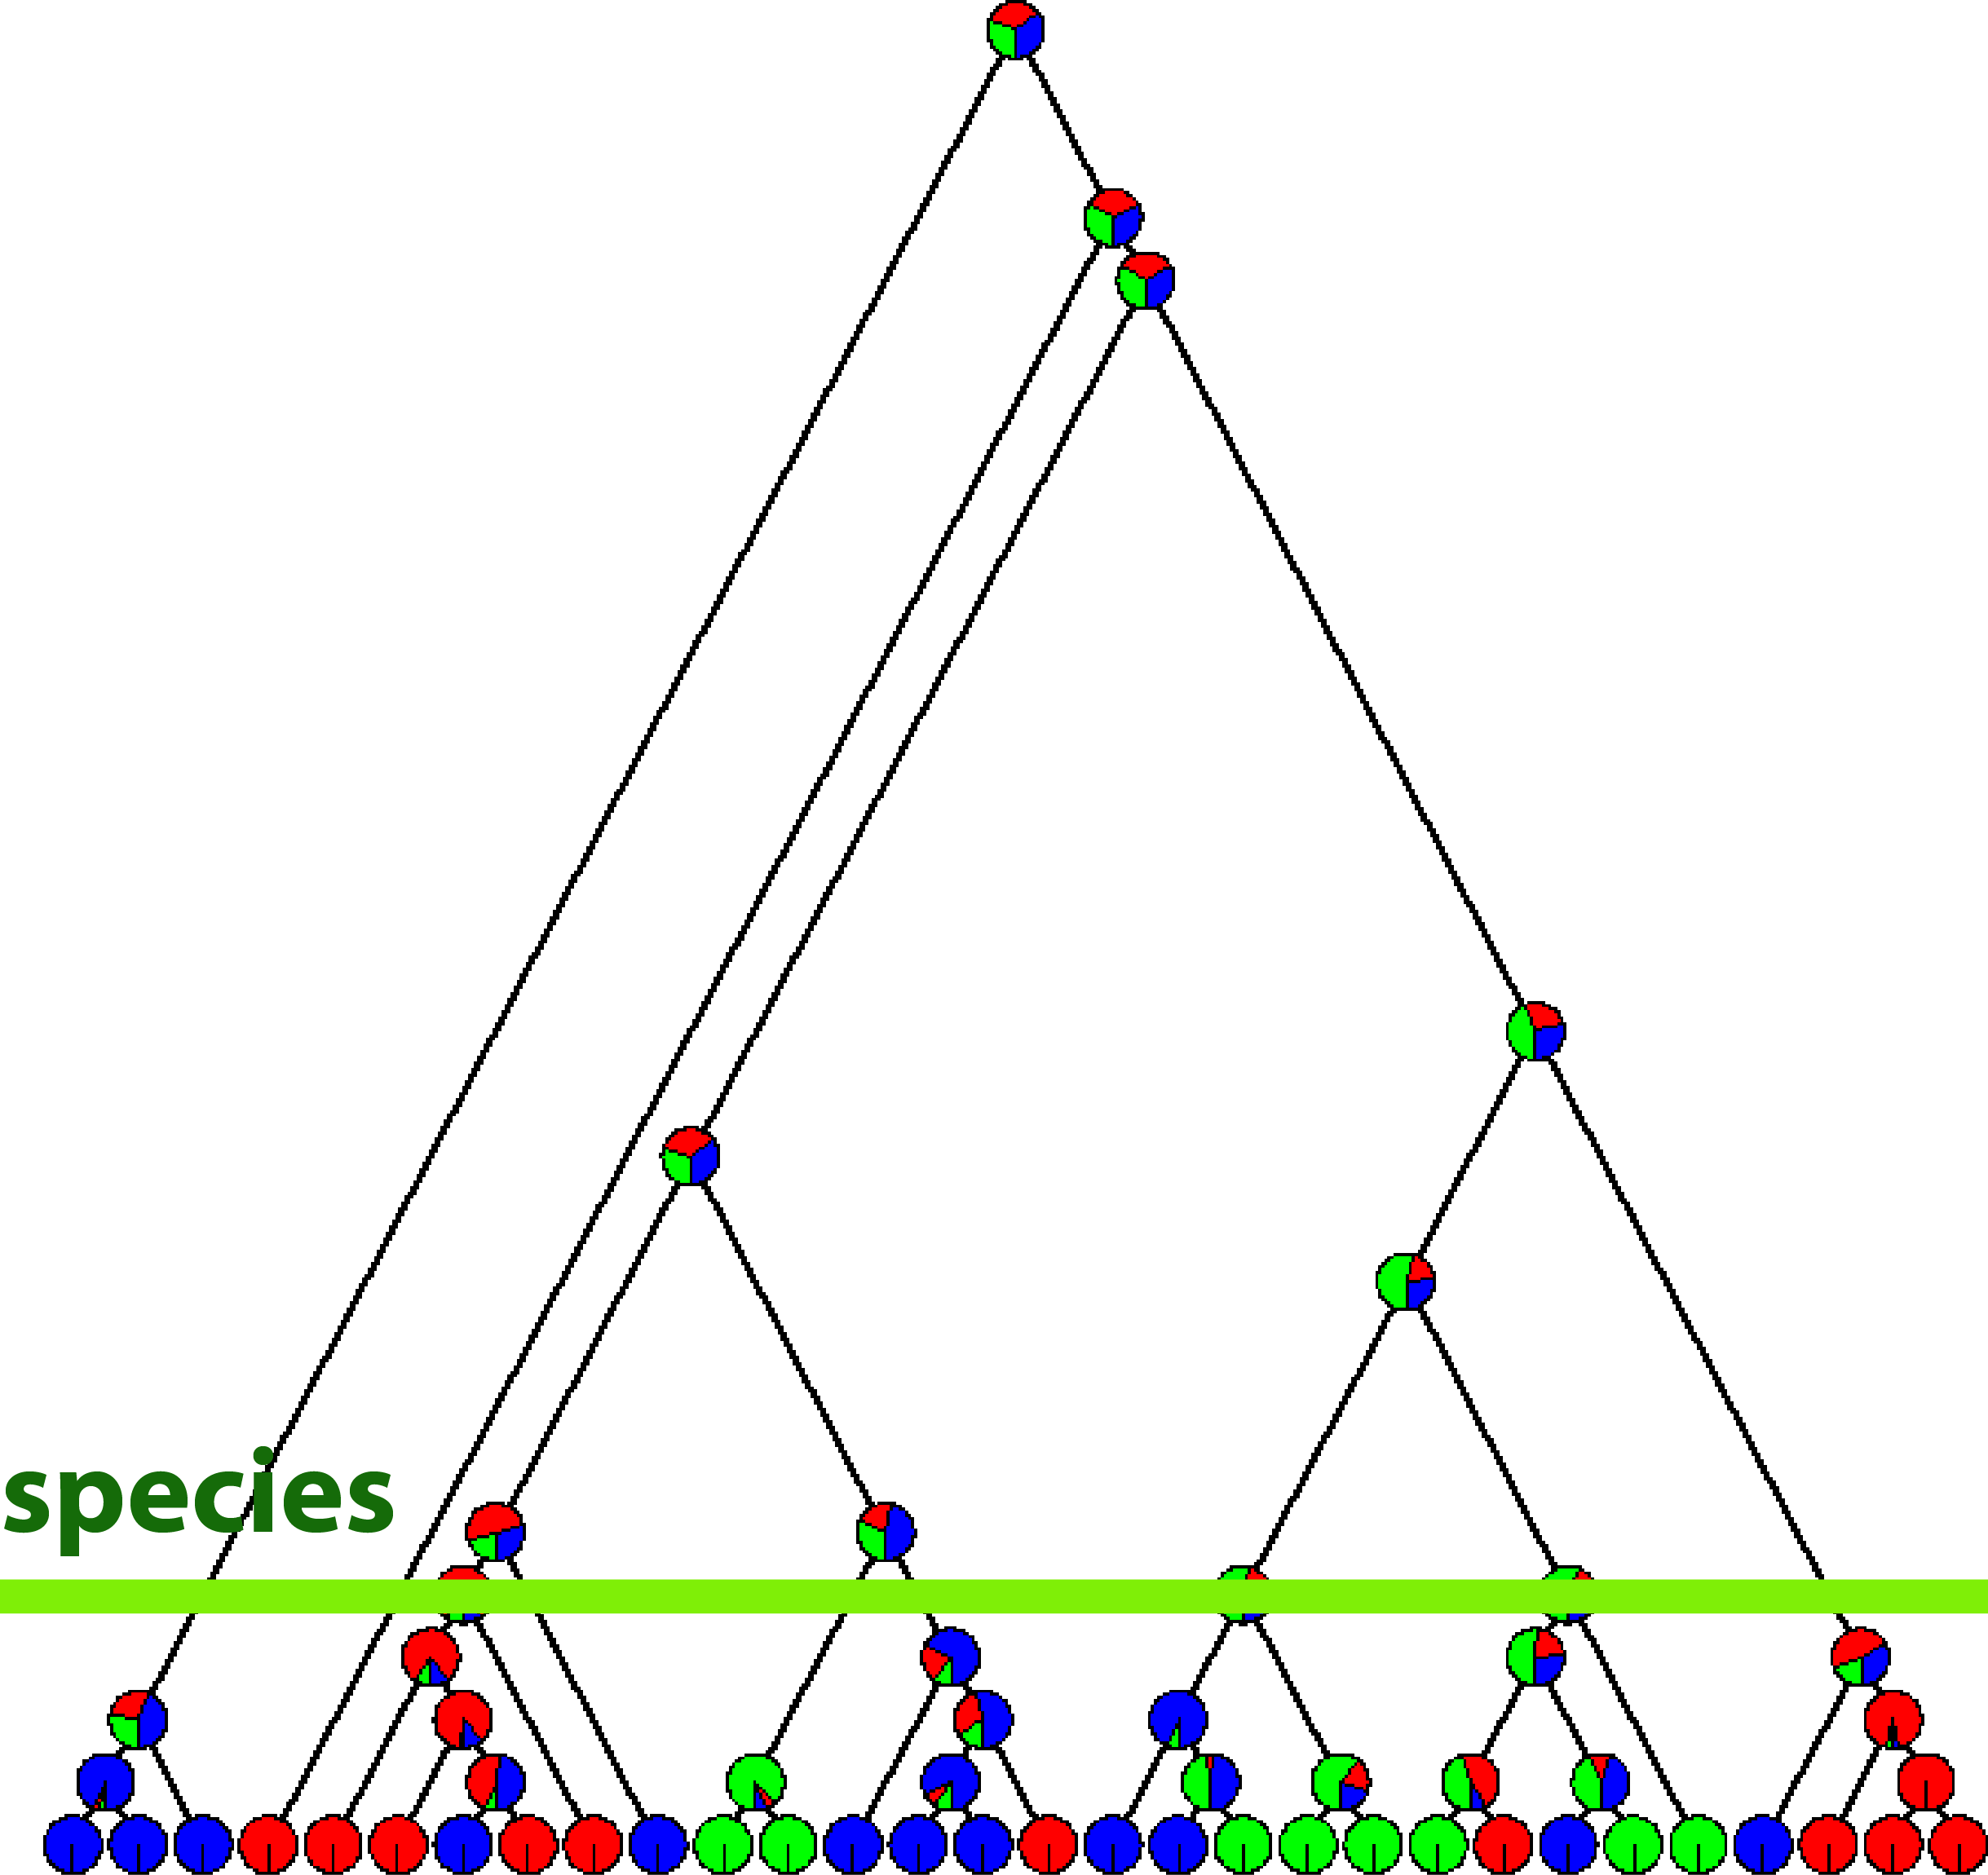
\includegraphics[width=\textwidth]{images/cladogram_species}
    \end{columns}  
\end{frame}

%
\begin{frame}
  \frametitle{Types of comparison}
    \begin{columns}[T] 
      \column{.5\textwidth} 
        \textcolor{RawSienna}{\textbf{Within genera/between species}}
        \begin{itemize}
	  \item comparison between groups of individuals
	  \item \textcolor{hutton_green}{what genome features show evidence of selective pressure?}
	  \item \textcolor{hutton_blue}{which features/changes are associated with species phenotype/adaptation?}      
        \end{itemize}
      \column{.5\textwidth}
        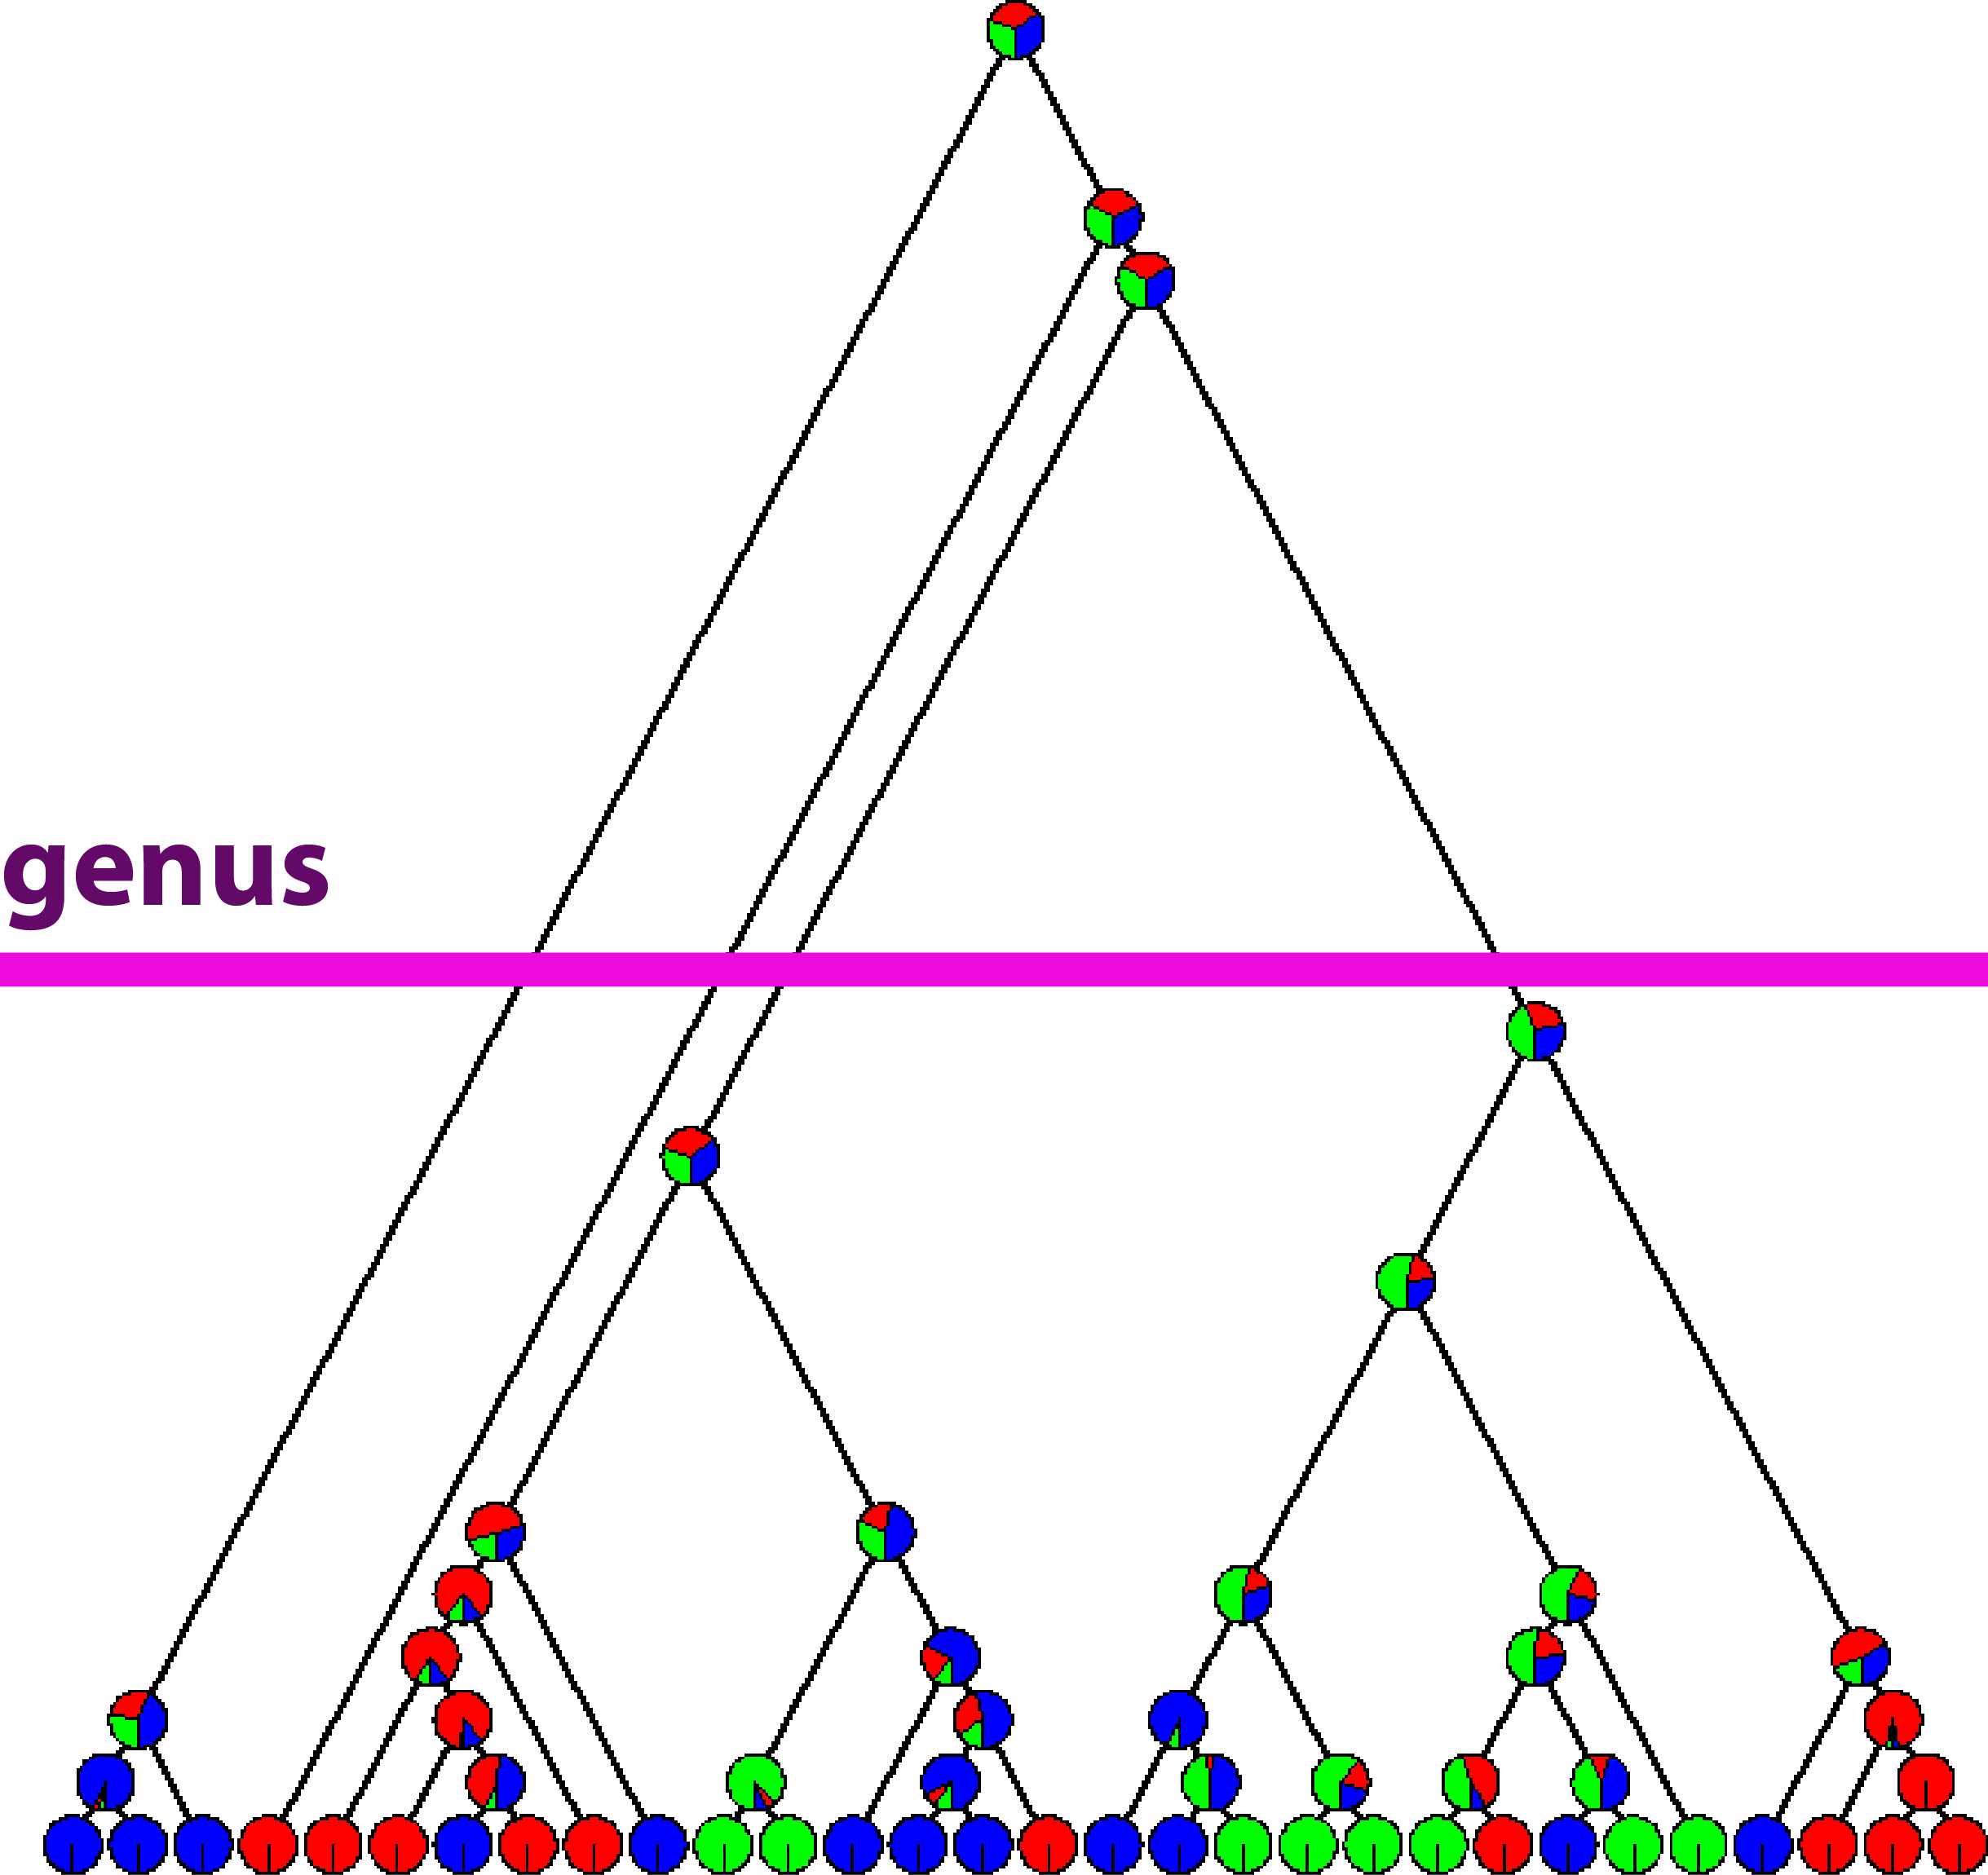
\includegraphics[width=\textwidth]{images/cladogram_genus}
    \end{columns}  
\end{frame}

%
\begin{frame}
  \frametitle{Types of comparison}
    \begin{columns}[T] 
      \column{.5\textwidth} 
        \textcolor{RawSienna}{\textbf{Between subgroups}}
        \begin{itemize}
          \item e.g. comparisons across many diverse individuals
          \item \textcolor{hutton_green}{what are the \textit{core set} of genome features that define a subgroup or genus?}
          \item \textcolor{hutton_blue}{what functions are present/absent between groups?}
        \end{itemize}
      \column{.5\textwidth}
        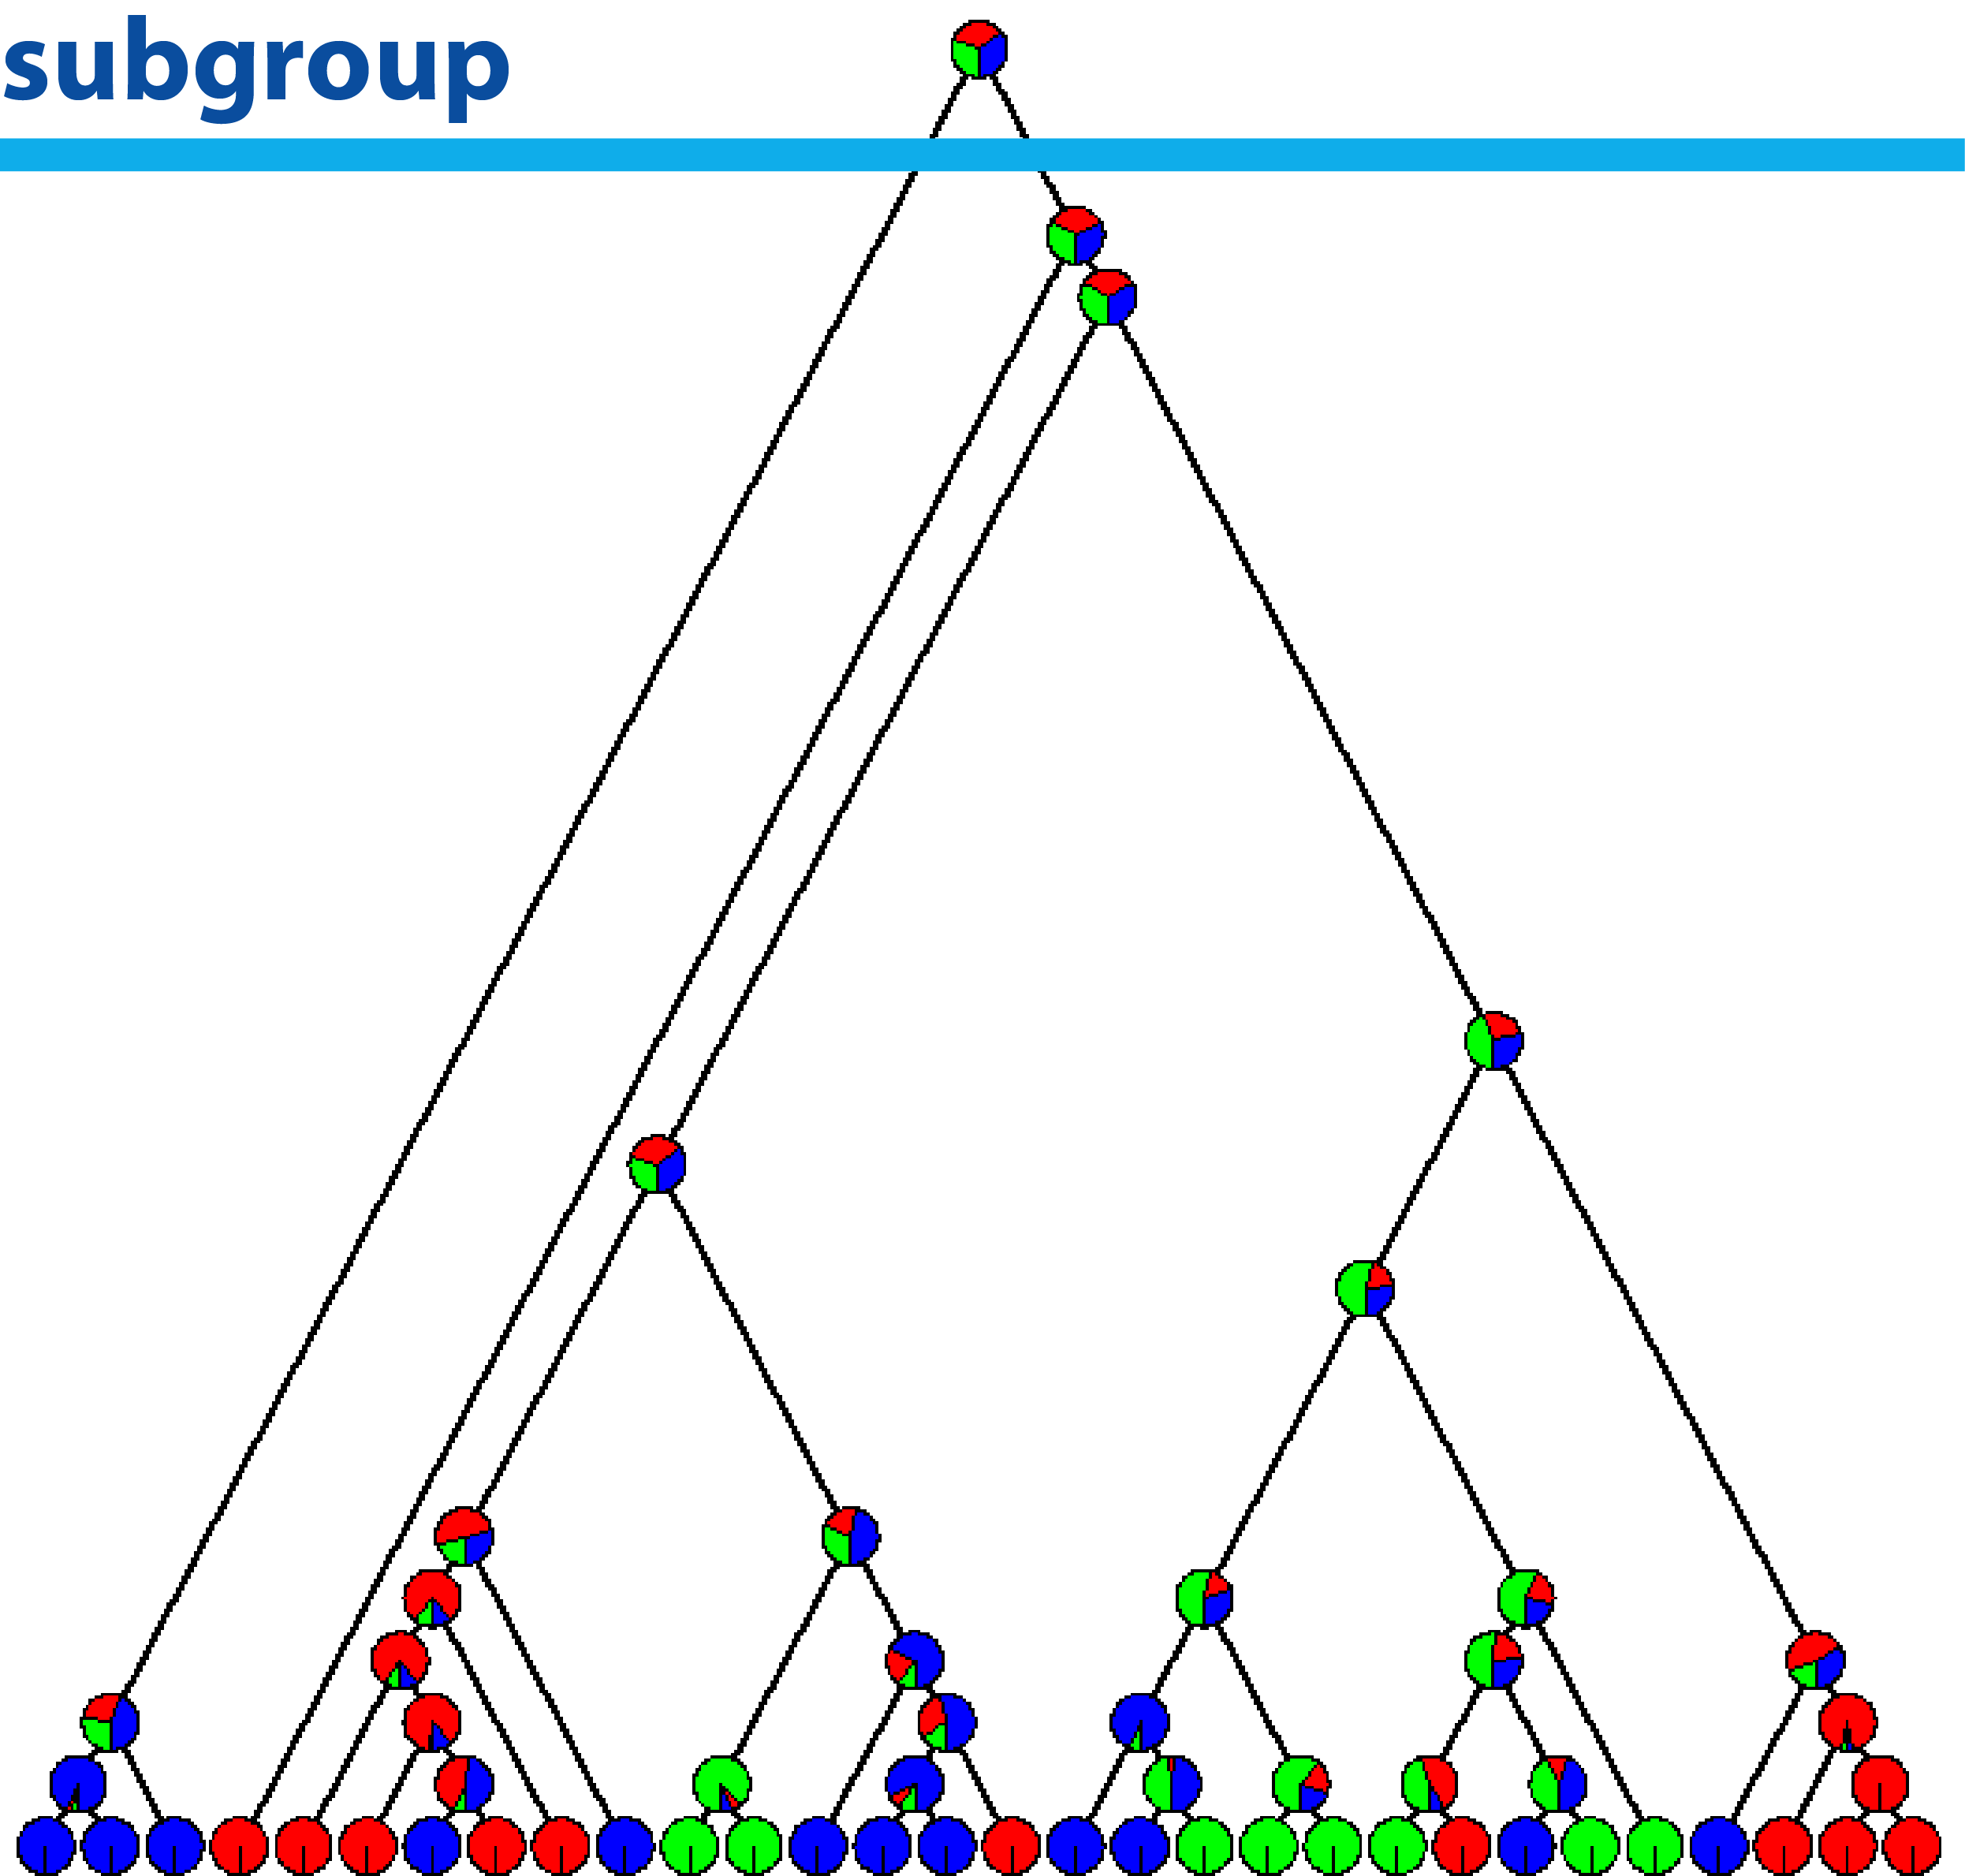
\includegraphics[width=\textwidth]{images/cladogram_subgroup}
    \end{columns}  
\end{frame}
%% ltee.tex
%% Author: Leighton Pritchard
%% Copyright: James Hutton Institute
%% Example slides: The Long-Term Evolution Experiment

%
\begin{frame}
  \frametitle{\textit{E. coli} LTEE
                   \footnote{\tiny{\href{http://dx.doi.org/10.1016/j.jmb.2009.09.052
}{Jeong \textit{et al}. (2009) \textit{J. Mol. Biol.} doi:10.1016/j.jmb.2009.09.052
}}}
                   \footnote{\tiny{\href{http://dx.doi.org/10.1038/nature08480
}{Barrick \textit{et al}. (2009) \textit{Nature} doi:10.1038/nature08480
}}}
                   \footnote{\tiny{\href{http://dx.doi.org/10.1126/science.1243357
}{Wiser \textit{et al}. (2013) \textit{Science} doi:10.1126/science.1243357
}}}}
    \begin{columns}[c] 
      \column{.6\textwidth} 
        \begin{itemize}
          \item \textcolor{RawSienna}{Run by the Lenski lab, Michigan State University since 1988 \\
          (\href{http://myxo.css.msu.edu/ecoli/}{http://myxo.css.msu.edu/ecoli/})}
          \item \textcolor{hutton_green}{12 flasks, citrate usage selection}
          \item \textcolor{hutton_blue}{$>$50,000 generations of \textit{E coli}!}
          \begin{itemize}
            \item Cultures propagated every day
            \item Every 500 generations (75 days), mixed-population samples stored
            \item Mean fitness estimated at 500 generation intervals
          \end{itemize}
        \end{itemize}
      \column{.4\textwidth}
        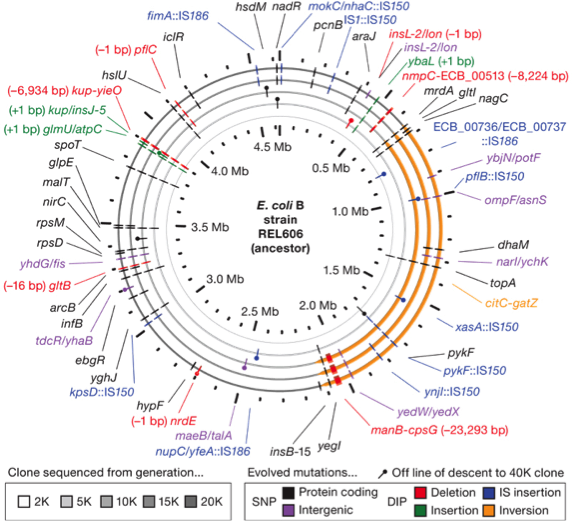
\includegraphics[width=\textwidth]{images/ltee_circular} \\
        
\includegraphics[width=\textwidth]{images/ltee_linear}        
    \end{columns}  
\end{frame}
%% neanderthal_2016.tex
%% Author: Leighton Pritchard
%% Copyright: James Hutton Institute
%% Example slides: Comparative Genomics In The News 2016

%
\begin{frame}
  \frametitle{Comparative genomics in the news
                   \footnote{\tiny{\href{http://www.bbc.co.uk/news/science-environment-35806992}{BBC News 15/3/2016
}}}
                   \footnote{\tiny{\href{http://dx.doi.org/10.1038/nature17405
}{Meyer \textit{et al}. (2016) \textit{Nature} doi:10.1038/nature17405
}}}
}
    \begin{columns}[c] 
      \column{.6\textwidth} 
        \begin{itemize}
          \item \textcolor{RawSienna}{Oldest DNA ever recovered from a human (430kya) - 0.1\% of genome}
          \item \textcolor{hutton_blue}{28 individuals, Sima de los Huesos, N. Spain}
          \item \textcolor{hutton_purple}{mitoDNA more similar to Siberian Denisovans than to modern humans}
          \item \textcolor{hutton_green}{Modern humans derived from wave out of Africa 250kya, with mitochondrial turnover?}
        \end{itemize}
      \column{.4\textwidth}
        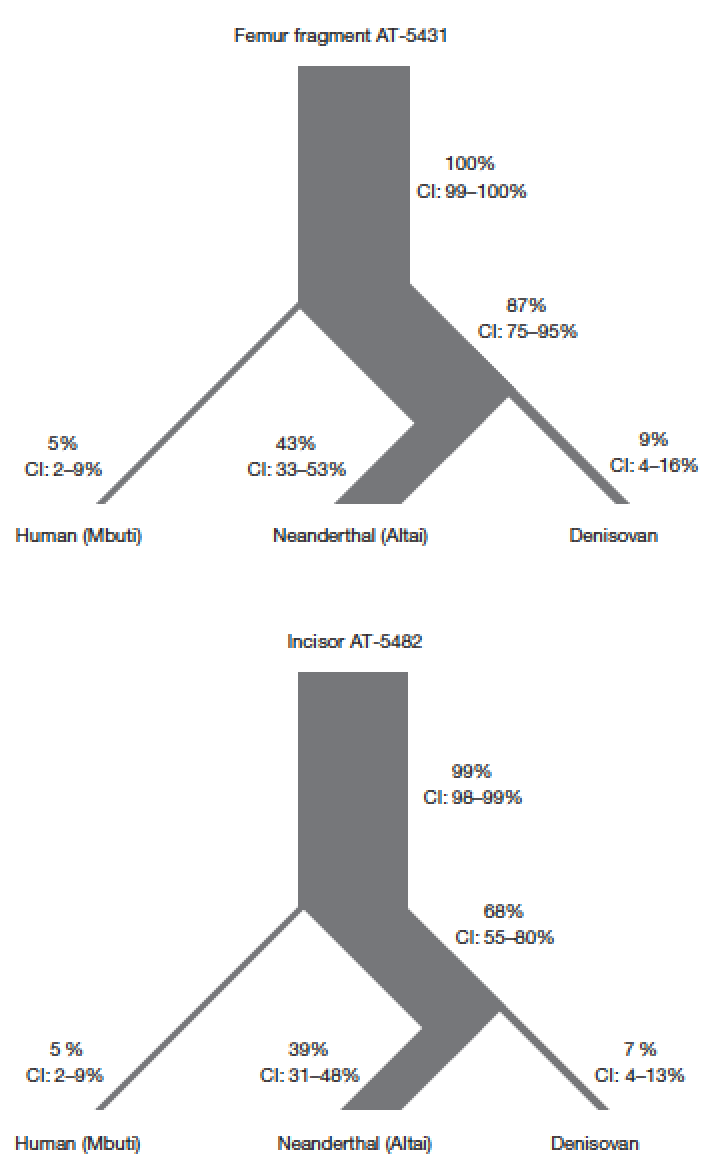
\includegraphics[width=\textwidth]{images/sima_shared} \\
        %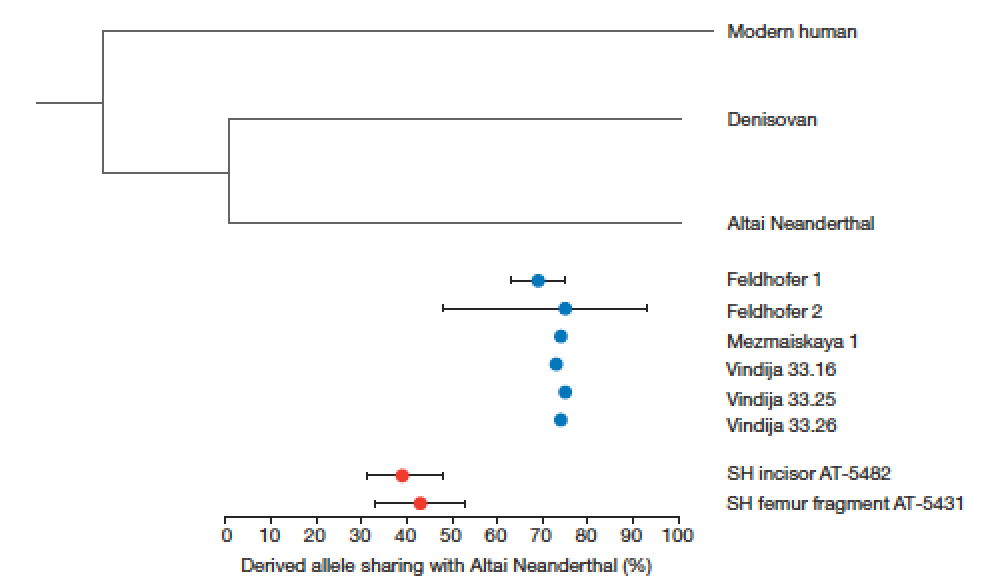
\includegraphics[width=\textwidth]{images/sima_tree}
    \end{columns}  
\end{frame}
%% SUBSECTION
%% Types of genome comparison (whole genome, features, etc.)
\subsection{Types of genome comparison}
%% comparison_types.tex
%% Author: Leighton Pritchard
%% Copyright: James Hutton Institute
%% Introductory slides: Types of comparison

%
\begin{frame}
  \frametitle{Levels of comparison}
  \textbf{Bulk Properties} \\
  \begin{itemize}  
    \item \textcolor{hutton_green}{chromosome/plasmid counts and sizes, nucleotide content, etc.}
  \end{itemize}    
  \textbf{Whole Genome Sequence} \\
    \begin{itemize}
      \item \textcolor{hutton_blue}{sequence similarity}
      \item \textcolor{hutton_blue}{organisation of genomic regions (synteny), etc.}
    \end{itemize}
  \textbf{Genome Features/Functional Components} \\
  \begin{itemize}
    \item \textcolor{hutton_purple}{numbers and types of features (genes, ncRNA, regulatory elements, etc.)}
    \item \textcolor{hutton_purple}{organisation of features (synteny, operons, regulons, etc.)}
    \item \textcolor{hutton_purple}{complements of features}
    \item \textcolor{hutton_purple}{selection pressure, etc.}
  \end{itemize}
\end{frame}

%%%
% SECTION: Making Comparisons
\section{Making Comparisons}

% SUBSECTION
% Computational comparisons
\subsection{In silico bulk genome comparisons}
%% bulk_genome_comparisons.tex
%% Author: Leighton Pritchard
%% Copyright: James Hutton Institute
%% Bulk genome comparisons

%
\begin{frame}
  \frametitle{Bulk genome comparisons}
  \Large{
    \textcolor{olive}{
      \textbf{
      You don't have to sequence genomes to compare them \\
      (but it helps) \\
      }
    }
  }
\end{frame}

%
\begin{frame}
  \frametitle{Genome comparisons predate NGS}
  \begin{itemize}
    \item Sequence data wasn't always cheap and abundant
    \item Practical, experimental genome comparisons were needed
  \end{itemize}
  \begin{center}
    
\includegraphics[width=0.7\textwidth]{images/land_before_time}
  \end{center}  
\end{frame}

%
\begin{frame}
  \frametitle{Bulk genome comparisons}
  \Large{
    \textcolor{olive}{
      \textbf{
      Calculate values for individual genomes, \\
      then compare them.
      }
    }
  }
  \normalsize{
        \begin{itemize}
         \item \textcolor{hutton_green}{Number of chromosomes}
         \item \textcolor{hutton_blue}{Ploidy}
         \item \textcolor{RawSienna}{Chromosome size}
         \item \textcolor{hutton_purple}{Nucleotide (A,C,G,T) frequency}        
        \end{itemize}
  }
\end{frame}

%
\begin{frame}
  \frametitle{Nucleotide frequency/genome size}
  Very easy to calculate from complete or draft genome sequence \\
  \begin{center}
    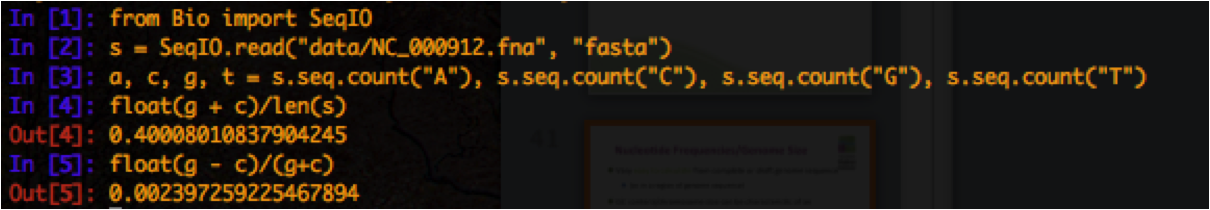
\includegraphics[width=\textwidth]{images/python_gc} \\
  \end{center}  
  GC content, chromosome size can be characteristic of an organism.
\end{frame}

%
\begin{frame}
  \frametitle{Genome Size}
  \begin{center}
    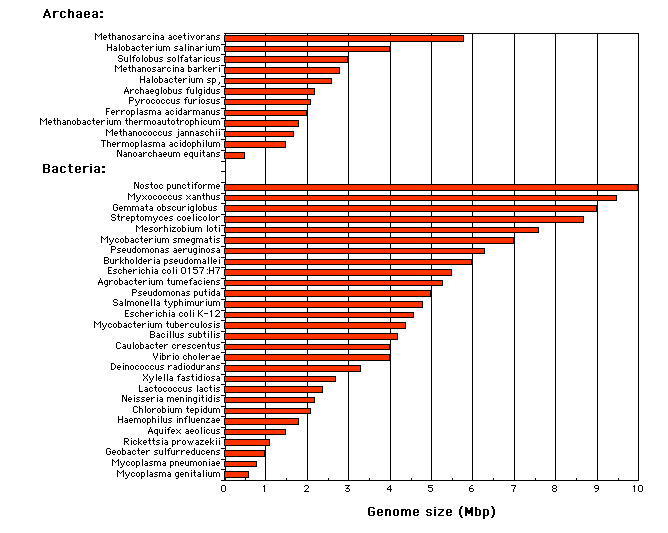
\includegraphics[height=0.7\textheight]{images/genome-sizes}
  \end{center}
\end{frame}

%
\begin{frame}
  \frametitle{Genome Size and GC\%}
  \begin{center}
    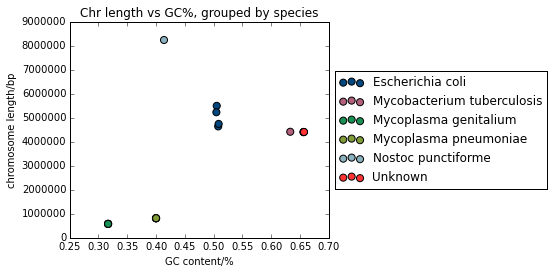
\includegraphics[width=\textwidth]{images/bacteria_gc_size}
  \end{center}
\end{frame}

%
\begin{frame}
  \frametitle{Blobology
  \footnote{\tiny{\href{http://dx.doi.org/10.1007/s13199-012-0154-6
}{Kumar \& Blaxter (2011) \textit{Symbiosis} doi:10.1007/s13199-012-0154-6
}}}
  \footnote{\tiny{\href{http://nematodes.org/bioinformatics/blobology/
}{http://nematodes.org/bioinformatics/blobology/
}}}  
  }
  Sequence data can be contaminated by other organisms
  \begin{itemize}
    \item \textcolor{hutton_green}{Host and symbiont DNA have different \%GC}
    \item \textcolor{hutton_green}{Host and symbiont DNA differ in coverage}
  \end{itemize}
      \begin{itemize}
        \item \textcolor{RawSienna}{Assemble genome}
        \item \textcolor{hutton_blue}{Map reads}
        \item \textcolor{hutton_purple}{Plot coverage against \%GC}
      \end{itemize}
\end{frame}

%
\begin{frame}
  \frametitle{Blobology
  \footnote{\tiny{\href{http://dx.doi.org/10.1007/s13199-012-0154-6
}{Kumar \& Blaxter (2011) \textit{Symbiosis} doi:10.1007/s13199-012-0154-6
}}}
  \footnote{\tiny{\href{http://nematodes.org/bioinformatics/blobology/
}{http://nematodes.org/bioinformatics/blobology/
}}}  
  }
  \begin{center}
    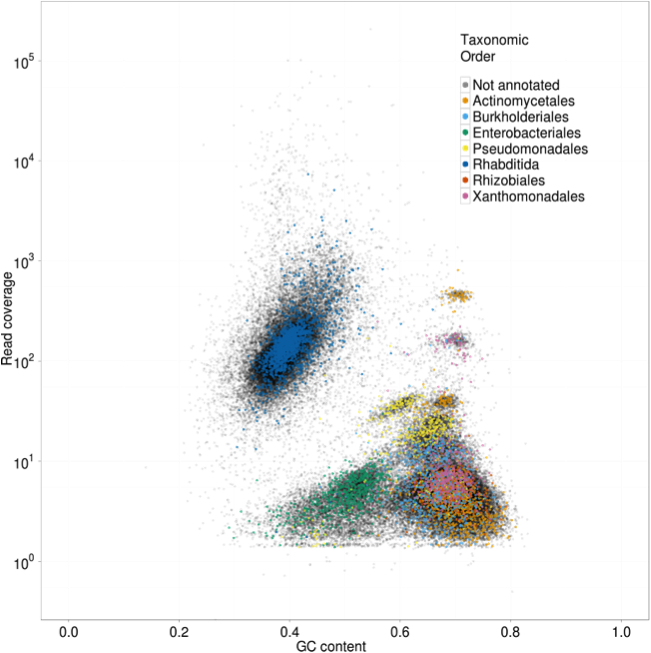
\includegraphics[height=0.7\textheight]{images/blobology}
  \end{center}
\end{frame}

%
\begin{frame}
  \frametitle{Nucleotide $k$-mers}
  Sequence data is necessary to determine $k$-mers/frequencies \\
  \textit{Not possible by experiment}
  \begin{itemize}
    \item \textcolor{hutton_green}{Nucleotides, $k=1$, 4x1-mers} \\
      \url{A, C, G, T}
    \item \textcolor{hutton_blue}{Dinucleotides, $k=2$, 16x2-mers} \\
      \url{AA, AC, AG, AT, CA, CC, CG, CT, GA, GC, GG, GT, TA, TC, TG, TT}
    \item \textcolor{RawSienna}{Triucleotides, $k=1$, 64x3-mers}
    \item \textcolor{hutton_purple}{$k$-nucleotides, $4^k$x$k$-mers}
  \end{itemize}  
\end{frame}

%
\begin{frame}
  \frametitle{$k$-mer spectra
  \footnote{\tiny{\href{http://dx.doi.org/10.1186/gb-2009-10-10-r108
}{Chor \textit{et al.} (2009) \textit{Genome Biol.} doi:10.1186/gb-2009-10-10-r108
}}}
  }
  \textcolor{RawSienna}{$k$-mer spectrum: frequency distribution of observed $k$-mer counts.} \\
  Most species have a unimodal $k$-mer spectrum
  \begin{center}
    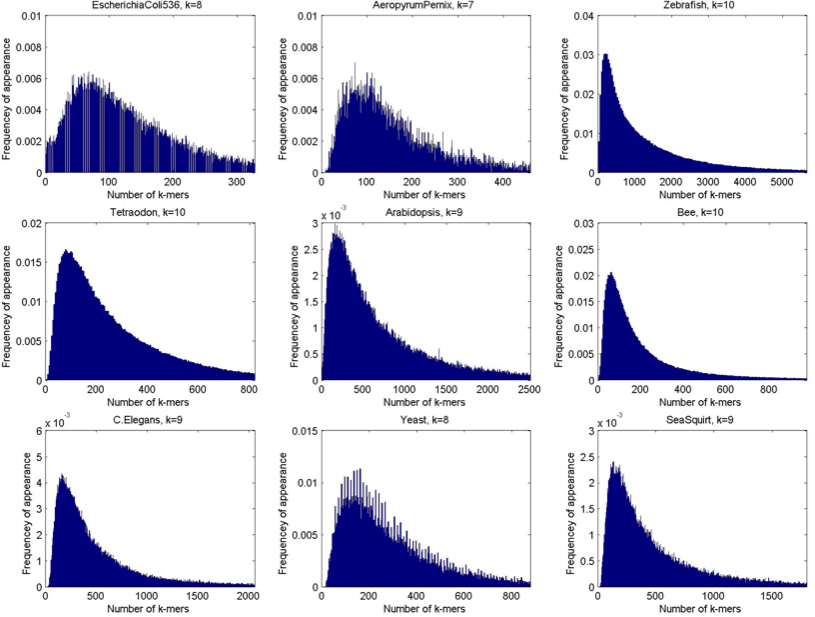
\includegraphics[height=0.6\textheight]{images/kmer_spectra} \\
  \end{center}  
\end{frame}

%
\begin{frame}
  \frametitle{$k$-mer spectra
  \footnote{\tiny{\href{http://dx.doi.org/10.1186/gb-2009-10-10-r108
}{Chor \textit{et al.} (2009) \textit{Genome Biol.} doi:10.1186/gb-2009-10-10-r108
}}}
  }
  \textcolor{RawSienna}{All mammals tested (and some other) species have \textit{multimodal $k$-mer spectra}} \\
  Genomic regions also differ in this property
  \begin{center}
    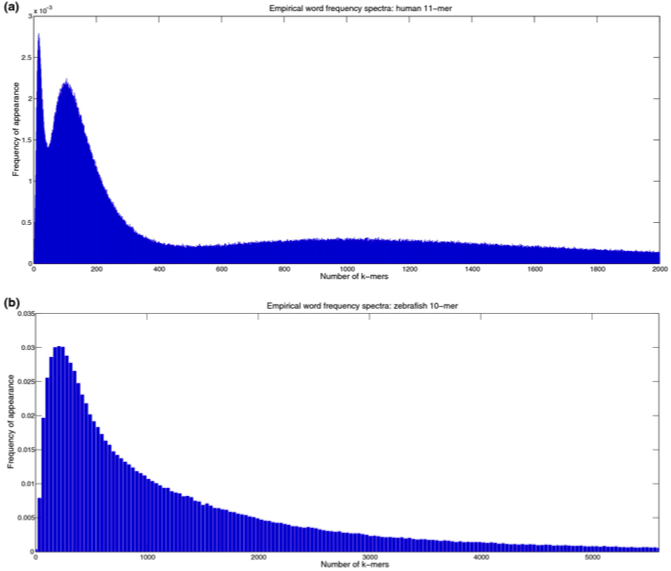
\includegraphics[height=0.4\textheight]{images/kmer_mammal1}
    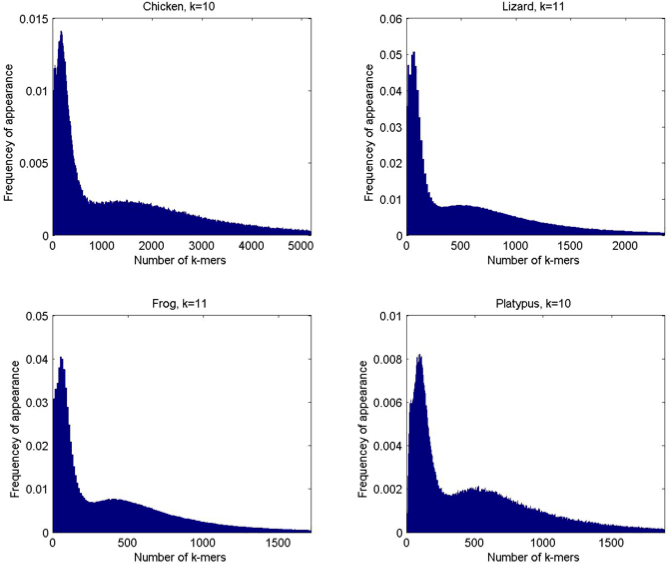
\includegraphics[height=0.4\textheight]{images/kmer_mammal2}    
  \end{center}  
\end{frame}

% SUBSECTION
% Whole genome comparisons
\subsection{Whole genome comparisons}
%% whole_genome_comparisons.tex
%% Author: Leighton Pritchard
%% Copyright: James Hutton Institute
%% Whole genome comparisons

%
\begin{frame}
  \frametitle{Whole genome comparisons}
  \Large{
    \textcolor{olive}{
      \textbf{
      Comparisons of one whole or draft genome with another \\
      ($\ldots$or many others)
      }
    }
  }
\end{frame}

%
\begin{frame}
  \frametitle{Whole genome comparisons}
  Minimum requirement: \textbf{two genomes} \\
  \begin{itemize}
    \item \textcolor{hutton_green}{Reference Genome}
    \item \textcolor{hutton_blue}{Comparator Genome}
  \end{itemize}
  The experiment produces a comparative result \textcolor{hutton_purple}{\textit{that is dependent on the choice of genomes}}.
\end{frame}

%
\begin{frame}
  \frametitle{Whole genome comparisons}
  Experimental methods mostly involve direct or indirect DNA hybridisation \\
  \begin{itemize}
    \item \textcolor{hutton_green}{DNA-DNA hybridisation (DDH)}
    \item \textcolor{hutton_blue}{Comparative Genomic Hybridisation (CGH)}
    \item \textcolor{hutton_purple}{Array Comparative Genomic Hybridisation (aCGH)}    
  \end{itemize}
\end{frame}

%
\begin{frame}
  \frametitle{Whole genome comparisons}
  Analogously, \textit{in silico} methods mostly involve sequence alignment \\
  \begin{itemize}
    \item \textcolor{hutton_green}{Average Nucleotide Identity (ANI)}
    \item \textcolor{hutton_blue}{Pairwise genome alignment}
    \item \textcolor{hutton_purple}{Multiple genome alignment}    
  \end{itemize}
\end{frame}

%
\begin{frame}
  \frametitle{DNA-DNA hybridisation (DDH)
  \footnote{\tiny{\href{http://dx.doi.org/10.1016/S0168-6445(00)00040-1
}{Morell\'{o}-Mora \& Amann (2011) \textit{FEMS Microbiol. Rev.} doi:10.1016/S0168-6445(00)00040-1
}}}
  }
  Several similar methods based on the same principle
  \begin{columns}[T] 
    \column{.4\textwidth} 
      \begin{itemize}
        \item \textcolor{hutton_green}{Denature gDNA mixture for organisms $A$, $B$}
        \item \textcolor{hutton_blue}{Allow gDNA to anneal; hybrids result}
      \end{itemize}
    \column{.6\textwidth}
      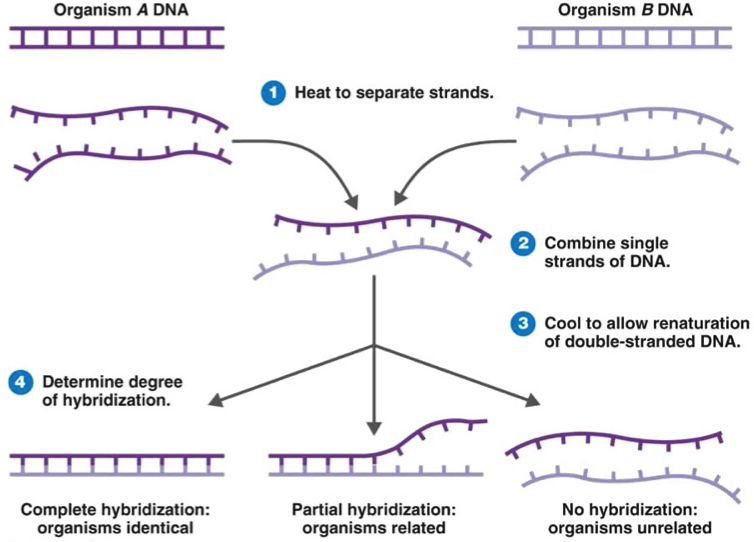
\includegraphics[width=\textwidth]{images/dna-dna_hyb}
  \end{columns}    
  \textcolor{hutton_green}{Reassociation of gDNA $\approx$ sequence similarity}
\end{frame}

%
\begin{frame}
  \frametitle{Average Nucleotide Identity (ANI)
  \footnote{\tiny{\href{http://dx.doi.org/10.1099/ijs.0.64483-0
}{Goris \textit{et al.} (2007) \textit{Int. J. System. Evol. Biol.} doi:10.1099/ijs.0.64483-0
}}}
  }
  Introduced as an \textit{in silico} substitute for DDH in 2007:
  \begin{columns}[T] 
    \column{.6\textwidth} 
      \begin{itemize}
        \item \textcolor{hutton_green}{70\% identity (DDH) = "gold standard" prokaryotic species boundary}
        \item \textcolor{hutton_blue}{70\% identity (DDH) $\approx$ 95\% identity (ANI)}
      \end{itemize}
    \column{.4\textwidth}
      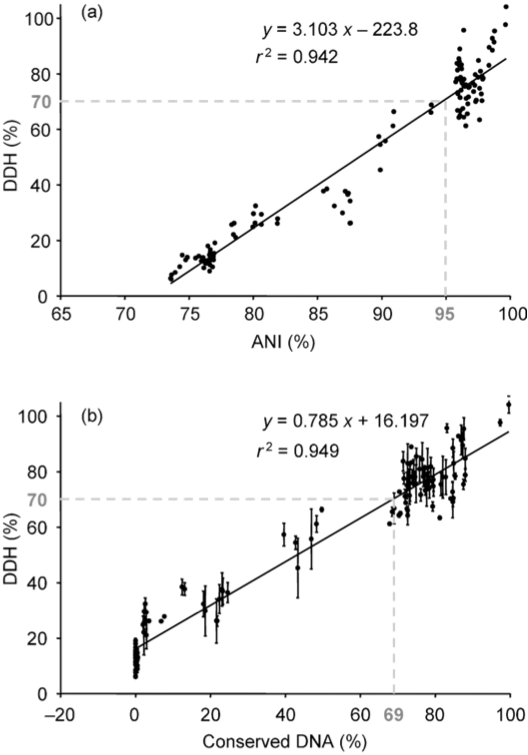
\includegraphics[width=\textwidth]{images/ani_ddh_equiv}
  \end{columns}    
\end{frame}

%
\begin{frame}
  \frametitle{Average Nucleotide Identity (ANI)
  \footnote{\tiny{\href{http://dx.doi.org/10.1073/pnas.0906412106
}{Richter \& Rossell\'{o}-M\'{o}ra \textit{et al.} (2009) \textit{Proc. Natl. Acad. Sci. USA} doi:10.1073/pnas.0906412106
}}}
  }
  ANIm and TETRA variants introduced in 2009:
  \begin{columns}[T] 
    \column{.5\textwidth} 
      \textcolor{RawSienna}{ANIm}
      \begin{enumerate}
        \item \textcolor{hutton_green}{Align sequences with NUCmer}
        \item \textcolor{hutton_purple}{ANI = mean identity of matches}
      \end{enumerate}
    \column{.5\textwidth}
      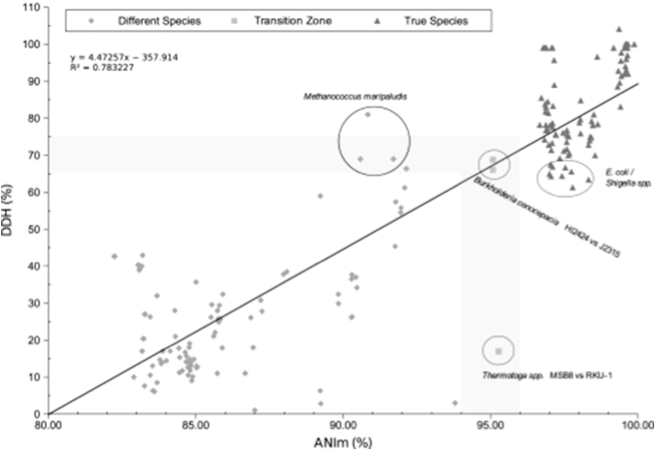
\includegraphics[width=\textwidth]{images/anim_ddh_equiv}
  \end{columns}    
  \textcolor{RawSienna}{TETRA} (a bulk measure!)
  \begin{enumerate}
    \item \textcolor{hutton_green}{Calculate 4-mer frequencies}
    \item \textcolor{hutton_blue}{Determine Z-score for 4-mer deviation from expected value, given \%GC content}
    \item \textcolor{hutton_purple}{TETRA = Pearson correlation coefficient of Z-scores}
  \end{enumerate}
\end{frame}

% ANIm in practice
\begin{frame}
  \frametitle{ANI in practice
    \footnote{\tiny{\href{http://dx.doi.org/10.1099/ijs.0.052944-0}{van der Wolf \textit{et al}. (2014) \textit{Int. J. Syst. Evol. Micr.} \textbf{64}:768-774 doi:10.1099/ijs.0.052944-0
    }}}
    \footnote{\tiny{\href{http://dx.doi.org/10.1039/C5AY02550H}{Pritchard \textit{et al}. (2016) \textit{Anal. Methods} \textbf{8}:12-24 doi:10.1039/C5AY02550H
    }}}
    }
  \begin{columns}[T]
    \begin{column}{5cm}
    \textit{Dickeya} species structure \\
      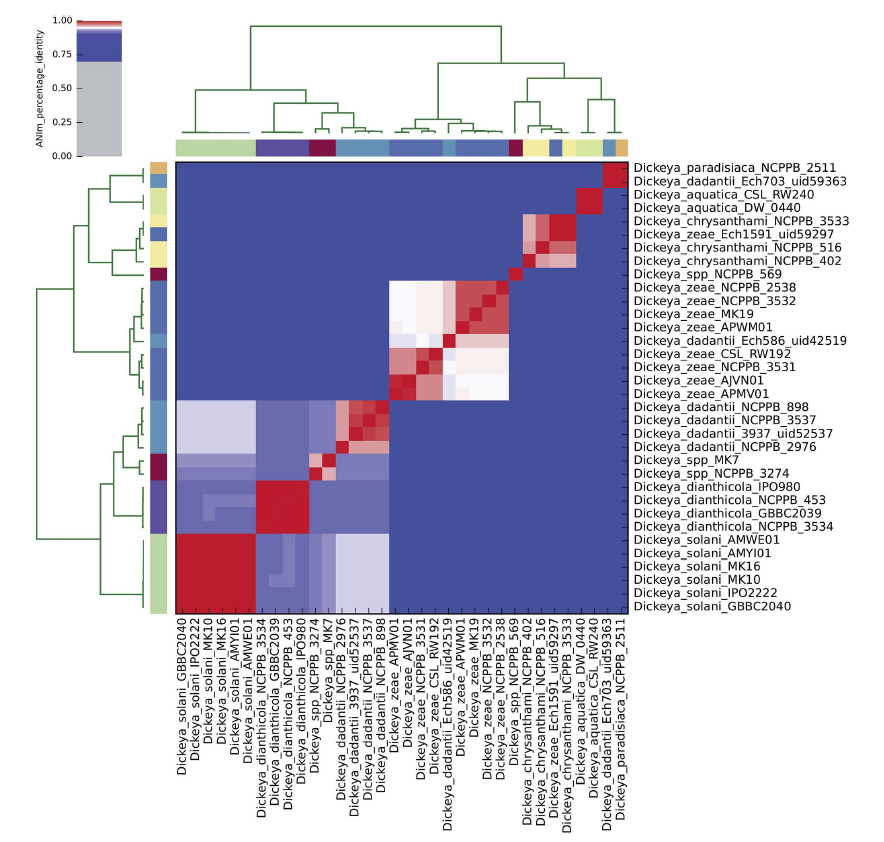
\includegraphics[width=\textwidth]{images/ANIm_dickeya}
    \end{column}
    \begin{column}{5cm}
    \textit{Pectobacterium} species structure:\\
      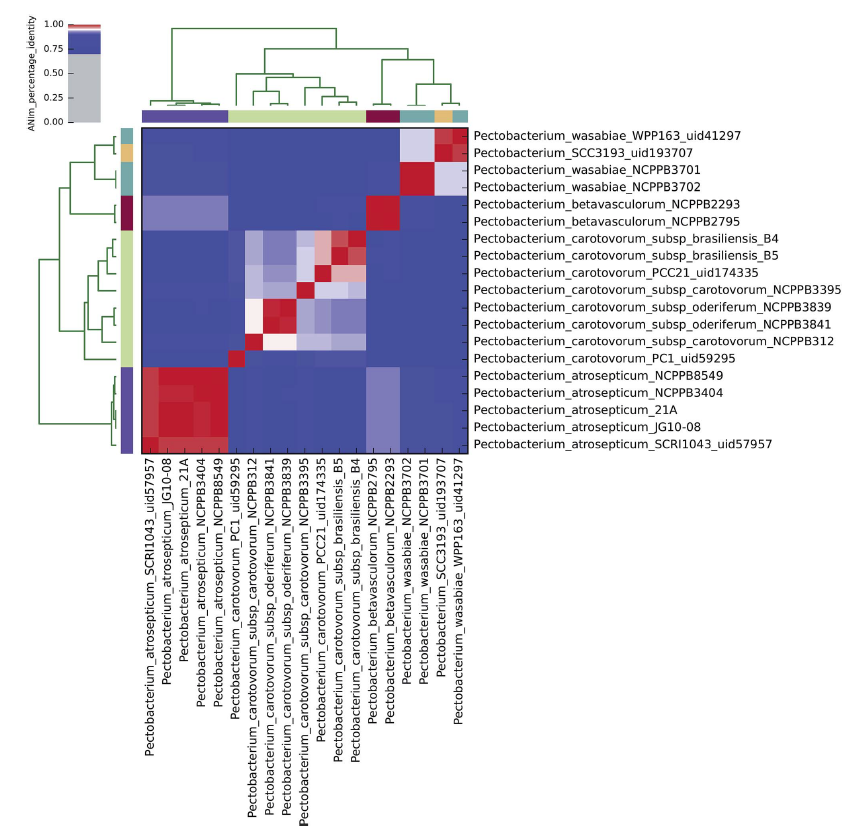
\includegraphics[width=\textwidth]{images/ANIm_pecto}
    \end{column}
  \end{columns}       
\end{frame}

%
\begin{frame}
  \frametitle{Pairwise genome alignments}
  \textcolor{olive}{Pairwise comparisons require alignment of similar regions.}
  \begin{center}
    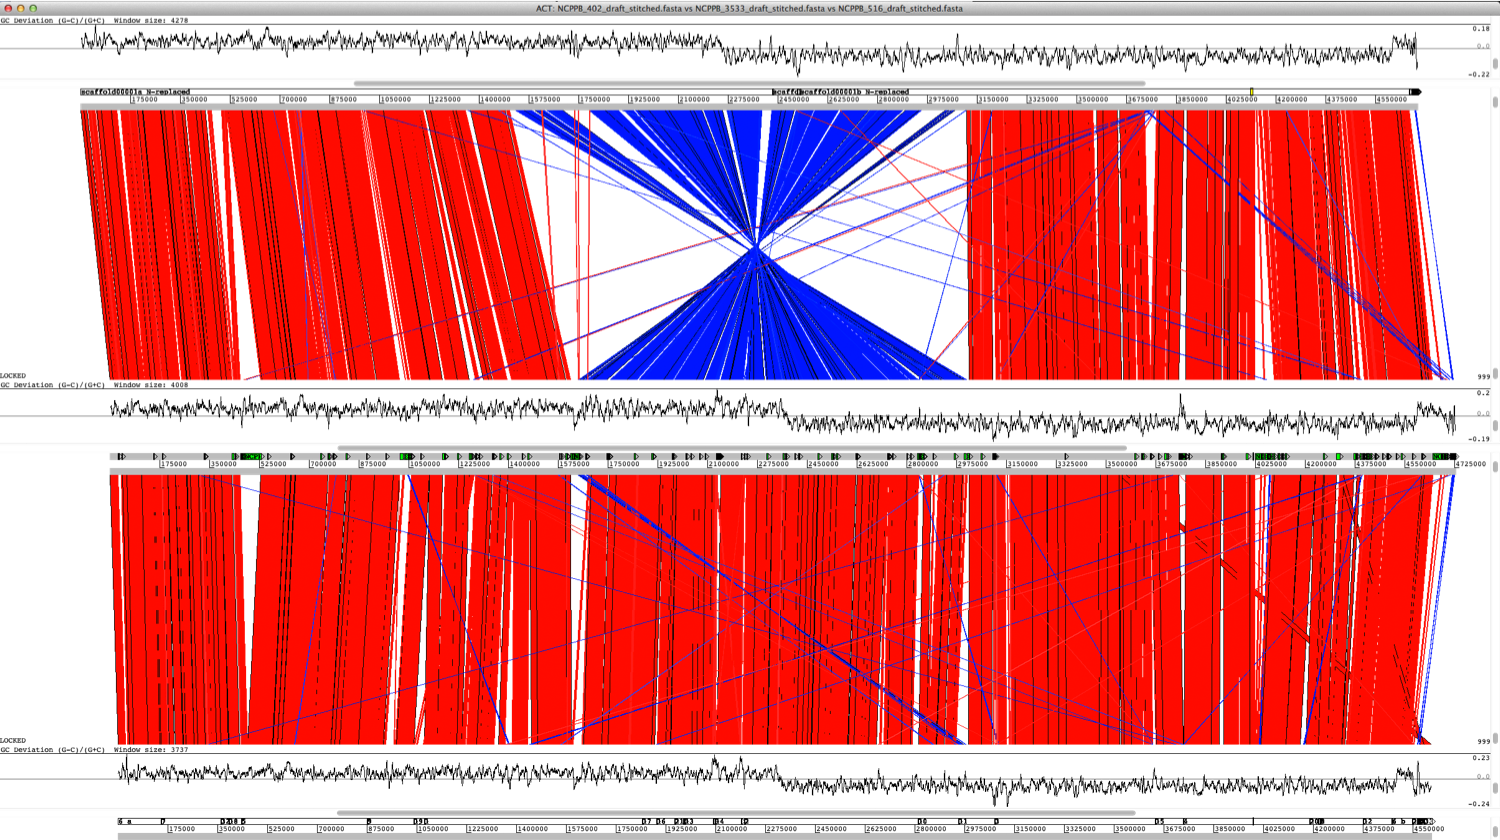
\includegraphics[width=\textwidth]{images/pairwise_genome_alignment}
  \end{center}  
\end{frame}

%
\begin{frame}
  \frametitle{Synteny and Collinearity}
  \textcolor{olive}{Genome rearrangements may occur post-divergence} \\
  Sequence similarity, and order of similar regions, may be conserved
  \begin{center}
    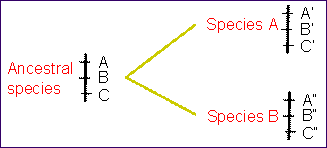
\includegraphics[width=0.5\textwidth]{images/collinear}    
    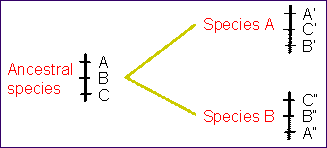
\includegraphics[width=0.5\textwidth]{images/synteny}
  \end{center}    
  \begin{itemize}
    \item \textcolor{hutton_blue}{\textit{collinear}} conserved elements lie in the same linear sequence
    \item \textcolor{hutton_purple}{\textit{syntenous} (or \textit{syntenic})} elements:
    \begin{itemize}
      \item (\textit{orig.}) lie on the same chromosome
      \item (\textit{mod.}) are collinear
    \end{itemize}
  \end{itemize}
  Evolutionary constraint (e.g. indicated by synteny) may indicate a functional constraint (and help determine \textit{orthology})
\end{frame}

%
\begin{frame}
  \frametitle{Alignment algorithms/programs}
  \textcolor{hutton_green}{I assume you're familiar with BLAST$\ldots$} \\
  \textcolor{RawSienna}{BLASTN and na\"{i}ve alignment algorithms are not appropriate for whole-genome alignment}:
  \begin{itemize}
    \item Needleman-Wunsch: optimal global alignment
    \item Smith-Waterman: optimal local alignment
  \end{itemize}
  \textcolor{hutton_blue}{Cannot handle rearrangement} \\
  \textcolor{hutton_purple}{Computationally expensive}  
\end{frame}

%
\begin{frame}
  \frametitle{Alignment algorithms/programs}
  \textcolor{hutton_green}{Many whole-genome alignment algorithms proposed} \\
  Handle genome-scale evolutionary processes, scalable \\~\\
  \begin{itemize}
    \item \href{http://www.bx.psu.edu/~rsharris/lastz/}{LASTZ (http://www.bx.psu.edu/$\sim$rsharris/lastz/)}
    \item \href{http://genome.ucsc.edu/goldenPath/help/blatSpec.html}{\textcolor{hutton_blue}{\textbf{BLAT} (http://genome.ucsc.edu/goldenPath)}}
    \item \href{http://mugsy.sourceforge.net/}{Mugsy (http://mugsy.sourceforge.net/)}
    \item \href{http://www.ncbi.nlm.nih.gov/blast/html/megablast.html}{\textcolor{red}{\textbf{megaBLAST} (http://www.ncbi.nlm.nih.gov/blast/)}}
    \item \href{http://mummer.sourceforge.net/}{\textcolor{red}{\textbf{MUMmer} (http://mummer.sourceforge.net/)}}
    \item \href{http://lagan.stanford.edu/lagan_web/index.shtml}{{\textcolor{hutton_blue}{LAGAN (http://lagan.stanford.edu/lagan\_web/index.shtml)}}}
    \item WABA, etc?
  \end{itemize}
\end{frame}

%
\begin{frame}
  \frametitle{megaBLAST
  \footnote{\tiny{Zhang \textit{et al.} (2000) \textit{J. Comp. Biol.} \textbf{7}(1-2): 203-214
}}
  \footnote{\tiny{Korf \textit{et al.} (2003) \textit{BLAST} O'Reilly \& Associates, Sebastopol, CA
}}
  }
  Optimised for:
  \begin{itemize}
    \item \textcolor{hutton_green}{speed and genome-level searching}
    \item \textcolor{hutton_blue}{queries on large sequence sets}: "query-packing"
    \item \textcolor{hutton_purple}{long alignments of very similar sequences} (\url{dc-megablast} for divergent sequences)
  \end{itemize}
  Uses Zhang et al. greedy algorithm, \textbf{not BLAST algorithm} \\~\\
  \textcolor{RawSienna}{BLASTN+ defaults to megaBLAST algorithm} \\
  (see \href{http://www.ncbi.nlm.nih.gov/blast/Why.shtml}{http://www.ncbi.nlm.nih.gov/blast/Why.shtml})
\end{frame}

%
\begin{frame}
  \frametitle{MUMmer
  \footnote{\tiny{\href{http://dx.doi.org/10.1186/gb-2004-5-2-r12
}{Kurtz \textit{et al.} (2004) \textit{Genome Biol.} doi:10.1186/gb-2004-5-2-r12
}}}
  }
  Conceptually completely different to BLAST/BLAT/megaBLAST \\
  \textcolor{RawSienna}{Uses \textit{suffix trees} for pattern matching}
  \begin{itemize}
    \item \textcolor{hutton_green}{Finds maximal exact matches}
    \item \textcolor{hutton_blue}{Memory use depends only on reference sequence size}
  \end{itemize}
  \begin{columns}[T] 
    \column{.5\textwidth} 
      \textcolor{hutton_purple}{Suffix Tree:}
      \begin{itemize}
        \item Constructed and searched in $O(n)$ time
        \item Useful algorithms are nontrivial
        \item \url{BANANA$}
      \end{itemize}
    \column{.5\textwidth}
      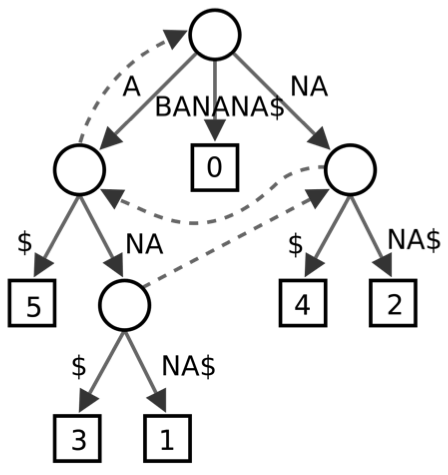
\includegraphics[width=0.75\textwidth]{images/suffix_tree}
  \end{columns}    
\end{frame}

%
\begin{frame}
  \frametitle{Pairwise genome alignments}
  \textcolor{hutton_green}{Which genomes should you align (or not bother with)?} \\
  \textcolor{RawSienna}{For reasonable analysis, genomes should}:
  \begin{itemize}
    \item derive from a sufficiently \textcolor{red}{recent} common ancestor, so that \textcolor{hutton_purple}{homologous regions can be identified}
    \item derive from a sufficiently \textcolor{red}{distant} common ancestor, so that \textcolor{hutton_purple}{biologically meaningful changes are likely to be found}
  \end{itemize}
\end{frame}

% Vibrio mimicus
\begin{frame}
  \frametitle{\textit{Vibrio mimicus} 
  \footnote{\tiny{\href{http://dx.doi.org/10.1073/pnas.1013825107}{Hasan \textit{et al}. (2010) \textit{Proc. Natl. Acad. Sci. USA} \textbf{107}:21134-21139 doi:10.1073/pnas.1013825107}}}
  }
  Chromosome C-II carries genes associated with environmental adaptation; C-I carries virulence genes.\\
  C-II has undergone extensive rearrangement; C-I has not.\\
  \begin{center}
    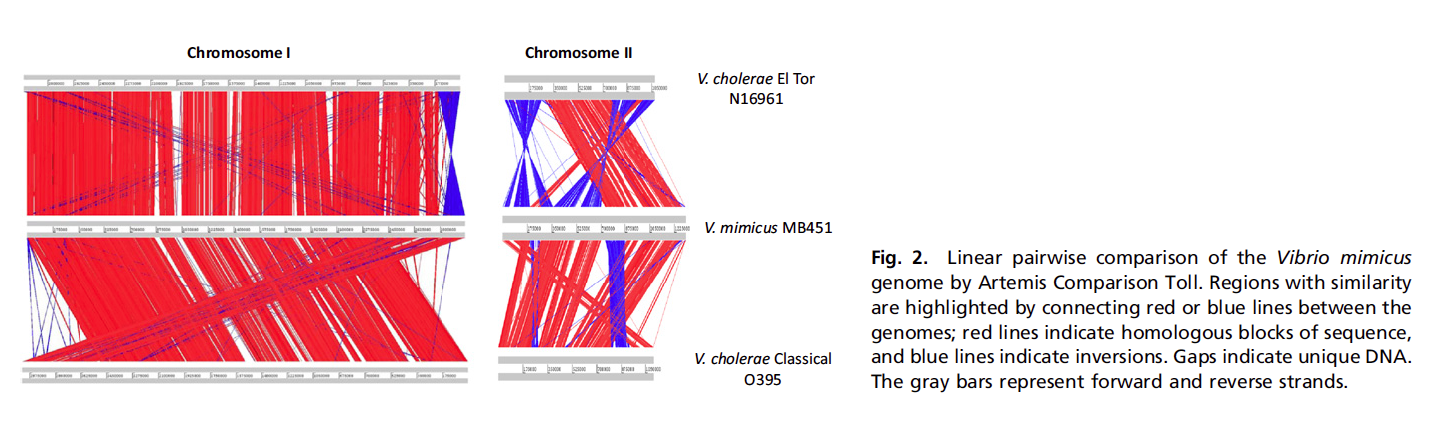
\includegraphics[width=1\textwidth]{images/v_mimicus}
  \end{center}    
  Suggests modularity of genome organisation, as a mechanism for adaptation (HGT, two-speed genome).
\end{frame}

% Serratia symbiotica
\begin{frame}
  \frametitle{\textit{Serratia symbiotica} 
  \footnote{\tiny{\href{http://dx.doi.org/10.1093/gbe/evr002}{Burke and Moran (2011) \textit{Genome Biol. Evol.} \textbf{3}:195-208 doi:10.1093/gbe/evr002}}}
  }
  \textit{S. symbiotica} is a recently evolved symbiont of aphids\\
  \textcolor{hutton_purple}{Massive genomic decay is an adaptation to the new environment.}\\
  \begin{center}
    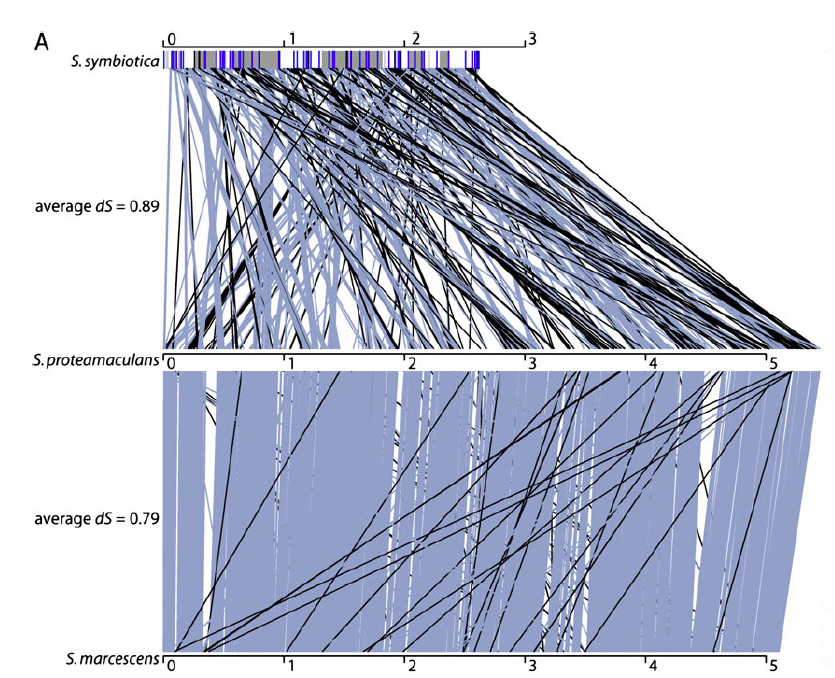
\includegraphics[width=0.75\textheight]{images/s_symbiotica}
  \end{center}    
\end{frame}

%
\begin{frame}
  \frametitle{Multiple genome alignments}
  \textcolor{olive}{Multiple genome alignments are ``harder'' than pairwise} \\
  \begin{itemize}
    \item Computationally difficult to produce
    \item \textcolor{red}{Lead to NP-complete optimisation problems!}
  \end{itemize}  
  \textcolor{hutton_green}{Solutions:} \textbf{heuristics}
  \begin{itemize}
    \item Progressive (build a tree, combine pairwise alignments)
    \item Iterative (realign initial sequences as new genomes added)
    \item \textcolor{hutton_blue}{Positional homology}
    \item \textcolor{hutton_purple}{\textit{Glocal} alignments}
  \end{itemize}  
\end{frame}

%
\begin{frame}
  \frametitle{Multiple genome alignment}
  Many tools use either positional homology or glocal alignment
  \begin{columns}[T] 
    \column{.5\textwidth} 
      \textcolor{olive}{Several tools available:}
      \begin{itemize}
        \item Mugsy: {\tiny\href{http://mugsy.sourceforge.net/}{(http://mugsy.sourceforge.net/)}}
        \item \textcolor{hutton_blue}{MLAGAN: {\tiny\href{http://lagan.stanford.edu/lagan_web/index.shtml}{(http://lagan.stanford.edu/lagan\_web/index.shtml)}}}
        \item TBA/MultiZ: {\tiny\href{http://www.bx.psu.edu/miller_lab/}{(http://www.bx.psu.edu/miller\_lab/)}}
        \item \textcolor{red}{\textbf{Mauve}: {\tiny\href{http://gel.ahabs.wisc.edu/mauve/}{(http://gel.ahabs.wisc.edu/mauve/)}}}
      \end{itemize}
    \column{.5\textwidth}
      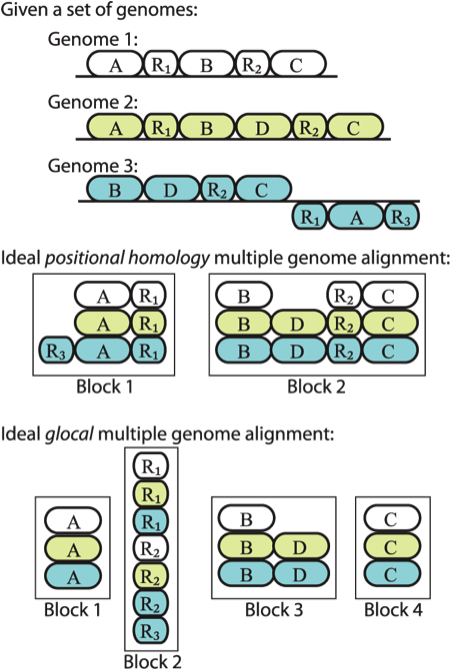
\includegraphics[width=0.75\textwidth]{images/poshom_v_glocal}
  \end{columns}    
\end{frame}

%
\begin{frame}
  \frametitle{MAUVE
  \footnote{\tiny{\href{http://dx.doi.org/10.1101/gr.2289704
}{Darling \textit{et al.} (2003) \textit{Genome Res.} doi:10.1101/gr.2289704
}}}
  }
  MAUVE alignment of nine enterobacterial genomes \\
  \textcolor{hutton_green}{Evidence for rearrangement of homologous backbone sequence}
  \begin{center}
    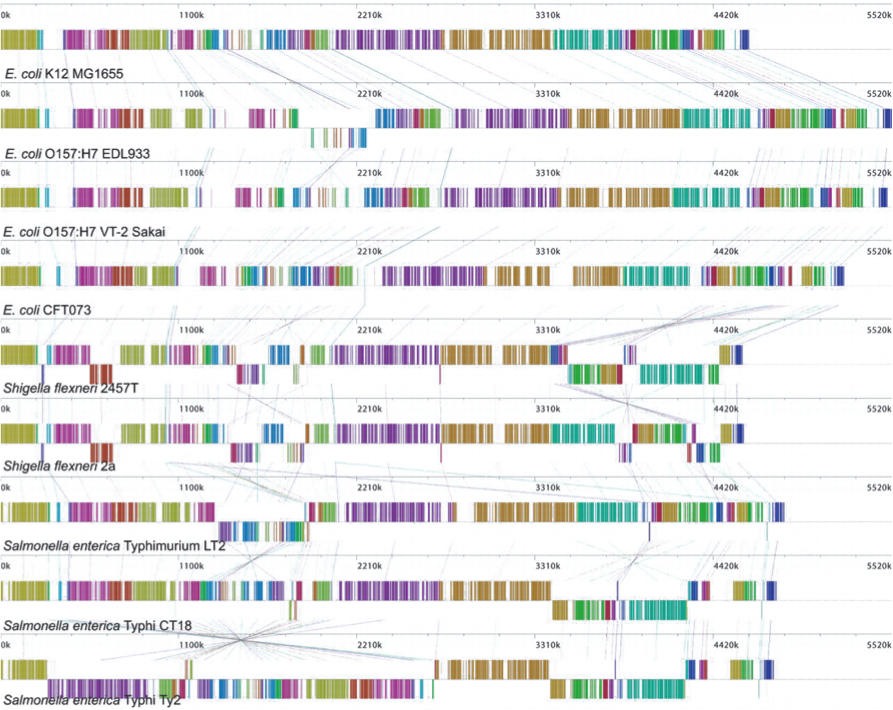
\includegraphics[height=0.6\textheight]{images/mauve_entero}
  \end{center}    
\end{frame}

%
\begin{frame}
  \frametitle{Draft genome alignment}
  \textcolor{olive}{High-throughput genome assemblies are often fragmented (contigs)} \\
  Contigs can be ordered (\textit{scaffolded}):
  \begin{itemize}
    \item \textcolor{hutton_blue}{without alignment}, by long or paired-end reads
    \item \textcolor{hutton_purple}{by alignment}, to complete \textit{reference} genomes or to other draft incomplete genomes
  \end{itemize}
  \begin{center}
    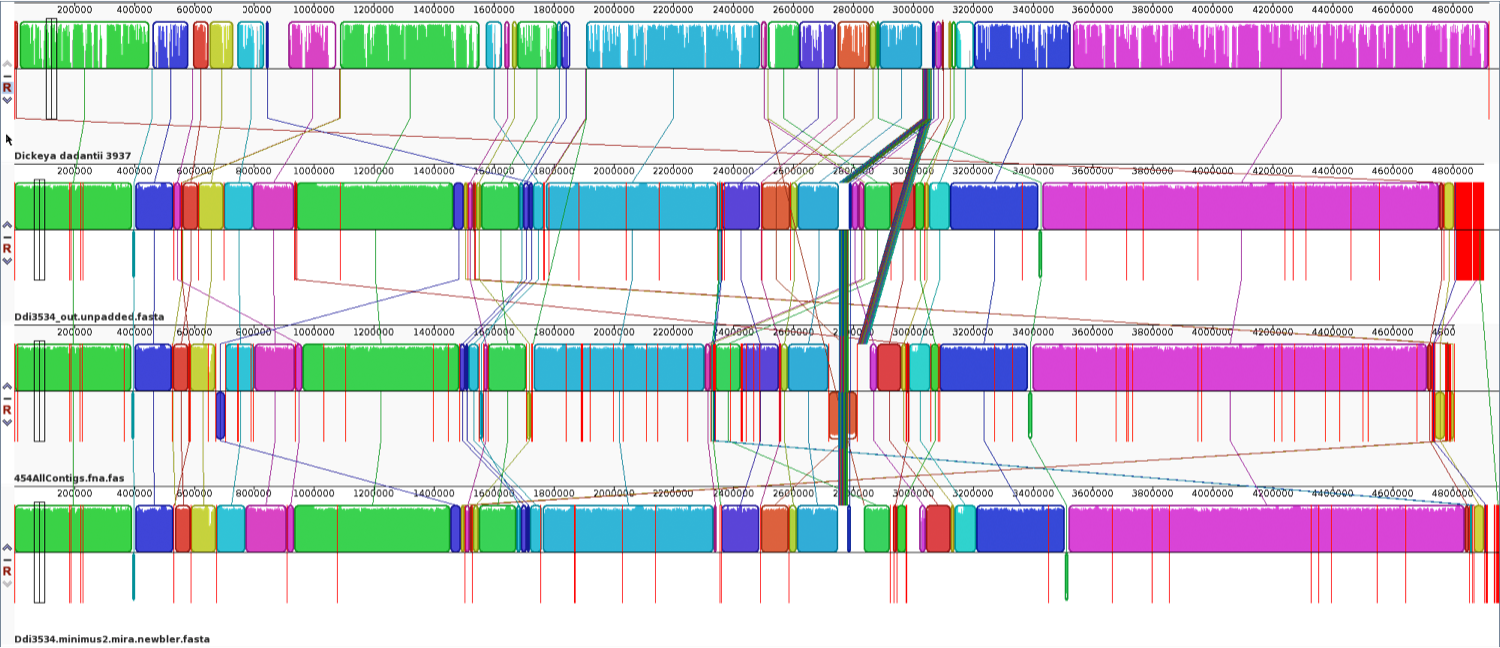
\includegraphics[width=\textwidth]{images/mauve_scaffolding}
  \end{center}    
\end{frame}

% DNA-DNA hybridisation
\begin{frame}
  \frametitle{Chromosome painting\footnote{\tiny{\href{http://dx.doi.org/10.1093/molbev/mst055}{Yahara \textit{et al}. (2013) \textit{Mol. Biol. Evol.} \textbf{30}:1454-1464 doi:10.1093/molbev/mst055}}}}
  ``Chromosome painting'' infers recombination-derived `chunks'\\
  Genome's haplotype constructed in terms of recombination events from a `donor' to a `recipient' genome\\
  \begin{center}
    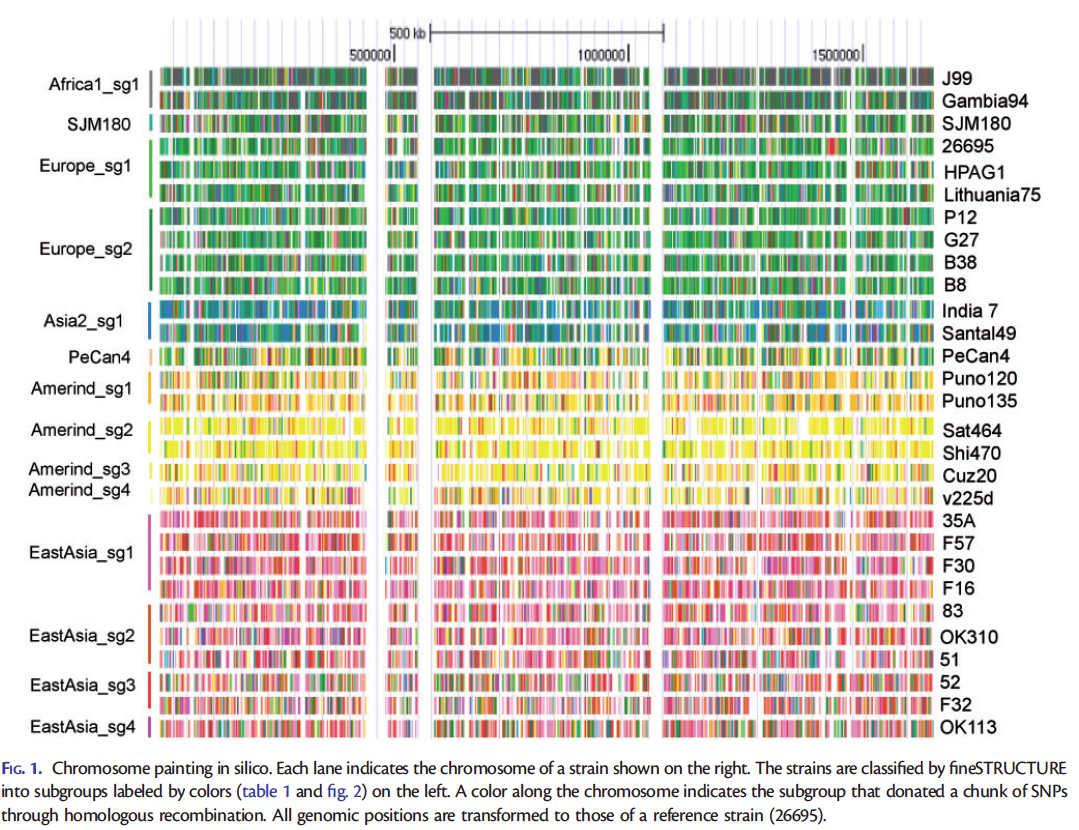
\includegraphics[width=0.7\textwidth]{images/chromosome_painting}
  \end{center}     
\end{frame}

% DNA-DNA hybridisation
\begin{frame}
  \frametitle{Chromosome painting\footnote{\tiny{\href{http://dx.doi.org/10.1093/molbev/mst055}{Yahara \textit{et al}. (2013) \textit{Mol. Biol. Evol.} \textbf{30}:1454-1464 doi:10.1093/molbev/mst055}}}}
  Recombination events summarised in a \textit{coancestry matrix}.\\
  \textit{H. pylori}: most within geographical bounds, but asymmetrical donation from Amerind/East Asian to European isolates.
  \begin{center}
    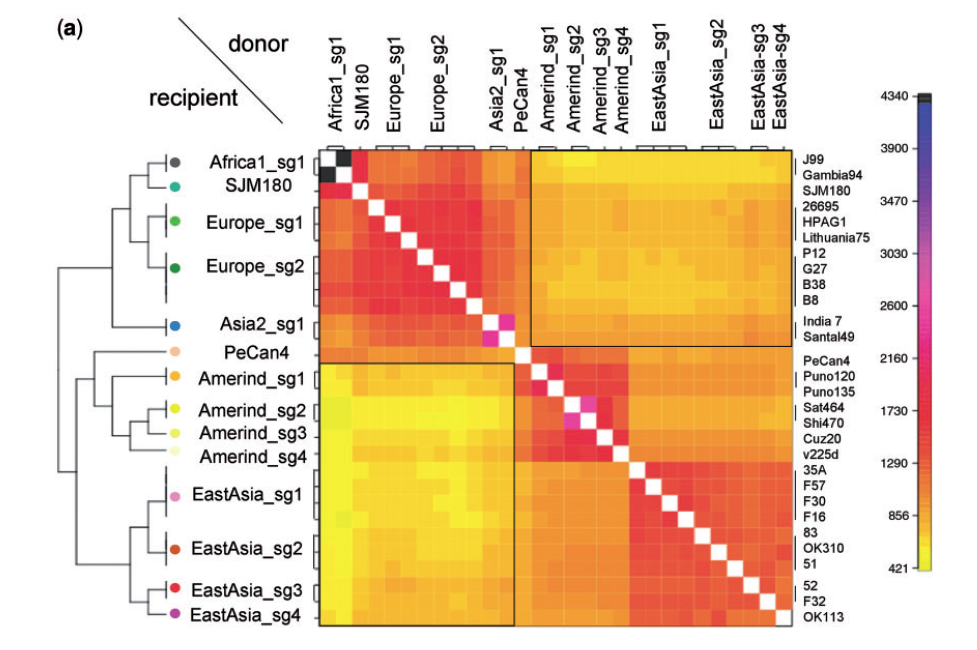
\includegraphics[width=0.75\textwidth]{images/coancestry}
  \end{center}     
\end{frame}

%
\begin{frame}
  \frametitle{Whole Genome Comparisons}
  \textcolor{RawSienna}{Physical and computational genome comparisons} \\
  \begin{itemize}
    \item Similar biological questions
    \item \textcolor{red}{$\therefore$ similar concepts}
  \end{itemize}  
  \textcolor{hutton_green}{Modern biology: lots of sequence data}
  \begin{itemize}
    \item Conservation $\approx$ evolutionary constraint
    \item \textcolor{hutton_blue}{Many choices of algorithms/software}
    \item \textcolor{hutton_purple}{Many choices of visualisation tools/software}
  \end{itemize}  
\end{frame}

% SUBSECTION
% Genome feature comparisons
\subsection{Genome feature comparisons}
%% genome_feature_comparisons.tex
%% Author: Leighton Pritchard
%% Copyright: James Hutton Institute
%% Genome feature comparisons

%
\begin{frame}
  \frametitle{Gene features}
  Significant substructure, especially in eukaryotes
  \begin{columns}[T] 
    \column{.4\textwidth} 
      \begin{itemize}
        \item translation start
        \item introns
        \item exons
        \item translation stop
        \item translation terminator
      \end{itemize}
    \column{.6\textwidth}
      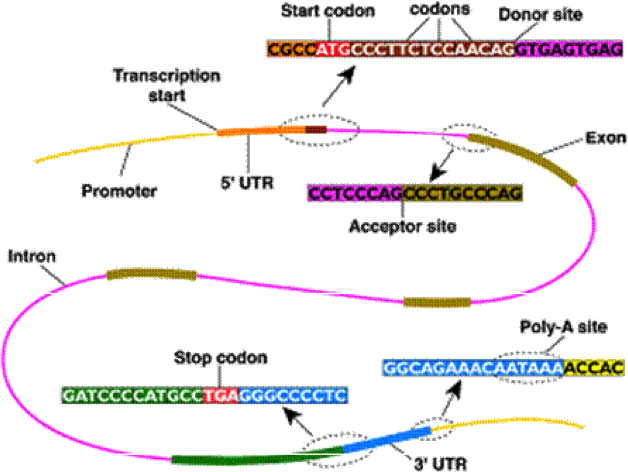
\includegraphics[width=\textwidth]{images/gene_feature}
  \end{columns}    
\end{frame}

%
\begin{frame}
  \frametitle{RNA features}
  \textcolor{hutton_blue}{RNA/ncRNA: characterised by complex secondary structure}
  \begin{columns}[T] 
    \column{.4\textwidth} 
      \begin{itemize}
        \item tRNA - transfer RNA
        \item rRNA - ribosomal RNA
        \item CRISPRs - prokaryotic defence, and genome editing
        \item many other functional classes, including enhancers
      \end{itemize}
    \column{.6\textwidth}
      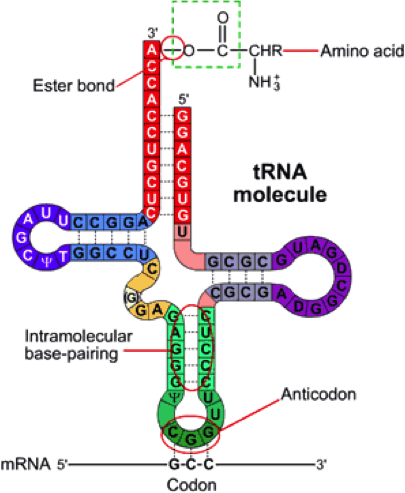
\includegraphics[height=0.7\textheight]{images/rna_feature}
  \end{columns}    
\end{frame}

%
\begin{frame}
  \frametitle{Regulatory features
  \footnote{\tiny{\href{http://dx.doi.org/10.1038/35052548
}{Pennacchio \& Rubin (2001) \textit{Nature Rev. Genet.} doi:10.1038/35052548
}}}  
  }
  \begin{itemize}
    \item transcription start sites (TSS)
    \item RNA polymerase (RNAp) binding sites
    \item transcription factor binding sites (TFBS)
    \item core, proximal and distal promoter regions
  \end{itemize}
  \begin{center}
    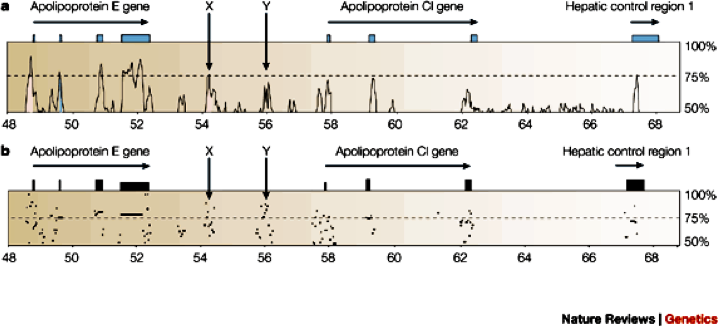
\includegraphics[width=0.8\textwidth]{images/regulatory_feature} \\
    \textcolor{hutton_green}{human vs mouse comparison}
  \end{center}    
\end{frame}

%
\begin{frame}
  \frametitle{Gene finding
  \footnote{\tiny{\href{http://dx.doi.org/10.1101/gr.088997.108
}{Liang \textit{et al.} (2009) \textit{Genome Res.} doi:10.1101/gr.088997.108
}}}
    \footnote{\tiny{\href{http://dx.doi.org/10.1038/nbt0807-883
}{Brent (2007) \textit{Nat. Biotech.} doi:10.1038/nbt0807-883
}}}
    \footnote{\tiny{\href{http://dx.doi.org/10.1186/1471-2105-5-59
}{Korf (2004) \textit{BMC Bioinf.} doi:10.1186/1471-2105-5-59
}}}
    }
  At genome scales, we need to automate functional prediction \\~\\    
  \textcolor{hutton_green}{Empirical (evidence-based) methods:}
  \begin{itemize}
    \item Inference from known protein/cDNA/mRNA/EST sequence
    \item Interference from mapped RNA reads (e.g. RNAseq)
  \end{itemize}
  \textcolor{hutton_blue}{\textit{Ab initio} methods:}
  \begin{itemize}
    \item Prediction on the basis of gene features (TSS, CpG islands, Shine-Dalgarno sequence, stop codons, nucleotide composition, etc.)
  \end{itemize}
  \textcolor{hutton_purple}{\textbf{Inference from genome comparisons/sequence conservation}}
\end{frame}

%
\begin{frame}
  \frametitle{Regulatory element finding
  \footnote{\tiny{\href{http://dx.doi.org/10.1186/1471-2105-12-238
}{Zhang \textit{et al.} (2011) \textit{BMC Bioinf.} doi:10.1186/1471-2105-12-238
}}}
    \footnote{\tiny{\href{http://dx.doi.org/10.1093/nar/gkt1123
}{Kilic \textit{et al.} (2013) \textit{Nucl. Acids Re.} doi:10.1093/nar/gkt1123
}}}
    \footnote{\tiny{\href{http://dx.doi.org/10.1016/j.gde.2005.05.002
}{Vavouri \& Elgar (2005) \textit{Curr. Op. Genet. Deve.} doi:10.1016/j.gde.2005.05.002
}}}
    }
  \textcolor{hutton_green}{Empirical (evidence-based) methods:}
  \begin{itemize}
    \item Inference from protein-DNA binding experiments
    \item Interference from co-expression
  \end{itemize}
  \textcolor{hutton_blue}{\textit{Ab initio} methods:}
  \begin{itemize}
    \item Identification of regulatory motifs (profile/other methods; TATA, $\sigma$-factor binding sites, etc.)
    \item Statistical overrepresentation of motifs
    \item Identification from sequence properties
  \end{itemize}
  \textcolor{hutton_purple}{\textbf{Inference from genome comparisons/sequence conservation}}
\end{frame}

% What do you align, and why?
\begin{frame}
  \frametitle{Equivalent genome features}
  \begin{center}
    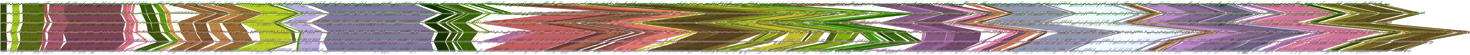
\includegraphics[width=1\textwidth]{images/collinear_zeae}  
  \end{center}
  When comparing two features (e.g. genes) between two or more genomes, there must be some basis for making the comparison. \\
  \textcolor{hutton_blue}{They have to be \textit{equivalent} in some way, such as:}
  \begin{itemize}
    \item common evolutionary origin
    \item functional similarity
    \item a family-based relationship
  \end{itemize}
  \textcolor{hutton_purple}{It's common to define equivalence of genome features in terms of evolutionary relationship.}
\end{frame}

% What do you align, and why?
\begin{frame}
  \frametitle{Why look at equivalent features?}
  \begin{center}
    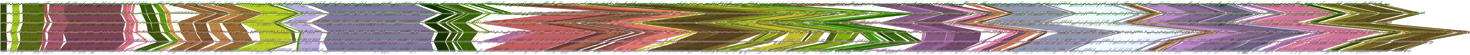
\includegraphics[width=1\textwidth]{images/collinear_zeae}  
  \end{center}
  \textbf{The real power of genomics is comparative genomics!}
  \begin{itemize}
    \item Makes catalogues of genome components comparable between organisms
    \item \textcolor{hutton_blue}{Differences, e.g. presence/absence of equivalents may support hypotheses for functional or phenotypic difference}
    \item \textcolor{hutton_green}{Can identify characteristic signals for diagnosis/epidemiology}
    \item \textcolor{hutton_purple}{Can build parts lists and wiring diagrams for systems and synthetic biology}
  \end{itemize}
\end{frame}

%
\begin{frame}
  \frametitle{Who let the -logues out?}
  \Large{
    \textcolor{olive}{
      \textbf{
      Genome features can have complex evolutionary relationships \\~\\
      We have precise terms to describe these relationships
      }
    }
  }
  \begin{center}
    
\includegraphics[width=0.4\textwidth]{images/who_let_the_dogs_out}
  \end{center}      
\end{frame}

%
\begin{frame}
  \frametitle{The -logues drop
  \footnote{\tiny{\href{http://dx.doi.org/10.2307/2412448
}{Fitch \textit{et al.} (1970) \textit{Syst. Zool.} doi:10.2307/2412448
}}}
  }
  How do we understand the relationships between features in more than one genome?
  \begin{itemize}
    \item \textcolor{hutton_green}{Functional similarity}: \textbf{analogy}
    \item \textcolor{hutton_blue}{Evolutionary common origin}: \textbf{homology, orthology, etc.}
    \item \textcolor{hutton_purple}{Evolutionary/functional/family relationship}: \textbf{paralogy}
  \end{itemize}
  \begin{center}
    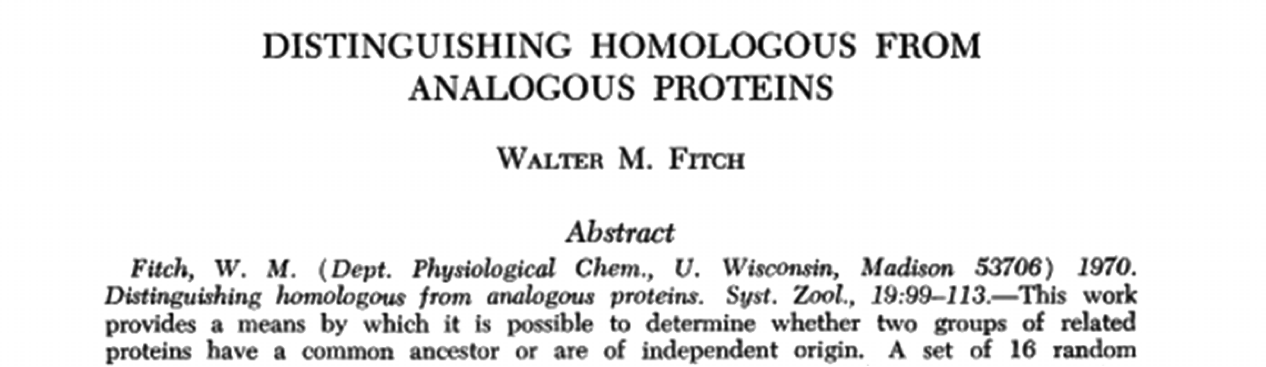
\includegraphics[width=\textwidth]{images/fitch}
  \end{center}    
\end{frame}

% 
\begin{frame}
  \frametitle{Who let the -logues out?}
  \begin{center}
    \includegraphics[width=1\textwidth]{images/logues1}  
  \end{center}  
\end{frame}

% 
\begin{frame}
  \frametitle{Who let the -logues out?}
  \begin{center}
    \includegraphics[width=1\textwidth]{images/logues2}  
  \end{center}  
\end{frame}

% 
\begin{frame}
  \frametitle{Who let the -logues out?}
  \begin{center}
    \includegraphics[width=1\textwidth]{images/logues3}  
  \end{center}  
\end{frame}

% 
\begin{frame}
  \frametitle{Orthology
    \footnote{\tiny{Storm \& Sonnhammer (2002) \textit{Bioinformatics} \href{http://dx.doi.org/10.1093/bioinformatics/18.1.92}{doi:10.1093/bioinformatics/18.1.92
    }}}
    }
  \begin{itemize}
    \item \textcolor{RawSienna}{Frequently abused/misused as a term}
    \item \textcolor{hutton_green}{``Orthology'' is an evolutionary relationship, bent into service as a functional descriptor}
    \item \textcolor{hutton_blue}{Orthology is strictly defined \textit{only for two species or clades}! (cf. OrthoMCL)}
    \item \textcolor{hutton_purple}{Orthology is not transitive: \\ ($A$ is an orthologue of $C$, and $B$ is an orthologue of $C$, does \textbf{not} imply that $A$ is an orthologue of $B$}
  \end{itemize}
  \textbf{All classifications of orthology/paralogy are inferences!}
\end{frame}

%
\begin{frame}
  \frametitle{The Ortholog Conjecture
    \footnote{\tiny{Nehrt \textit{et al.} (2011) \textit{PLoS Comp. Biol.} \href{http://dx.doi.org/10.1371/journal.pcbi.1002073}{doi:10.1371/journal.pcbi.1002073
    }}}  
    \footnote{\tiny{Chen \textit{et al.} (2012) \textit{PLoS Comp. Biol.} \href{http://dx.doi.org/10.1371/journal.pcbi.1002784}{doi:10.1371/journal.pcbi.1002784
    }}}  
  }
  \Large{
    \textcolor{olive}{
      \textbf{
      Without duplication, a gene product is unlikely to change its basic function, because this would lead to loss of the original function, and this would be harmful.
      }
    }
  }
\end{frame}

% 
\begin{frame}
  \frametitle{Why focus on orthologues?
    \footnote{\tiny{Chen and Zhang (2012) \textit{PLoS Comp. Biol.} \href{http://dx.doi.org/10.1371/journal.pcbi.1002784}{doi:10.1371/journal.pcbi.1002784
    }}}  
    \footnote{\tiny{Dessimoz (2011) \textit{Brief. Bioinf.} \href{http://dx.doi.org/10.1093/bib/bbr057}{doi:10.1093/bib/bbr057
    }}}
    \footnote{\tiny{Altenhoff and Dessimoz (2009) \textit{PLoS Comp. Biol.} \textbf{5}:e1000262 \href{http://dx.doi.org/10.1371/journal.pcbi.1000262}{doi:10.1371/journal.pcbi.1000262
    }}}
  }
  Formalisation of the idea of \textit{corresponding genes} in different organisms. \\
  \textcolor{hutton_blue}{Orthologues serve two purposes:}
  \begin{itemize}
    \item \textcolor{hutton_green}{\textbf{Evolutionary equivalence}}
    \item \textcolor{hutton_purple}{\textbf{Functional equivalence}} (``The Ortholog Conjecture'')
  \end{itemize}
  Applications in comparative genomics, functional genomics and phylogenetics. \\
  \textcolor{RawSienna}{Over 30 databases attempt to describe orthologous relationships} (\href{http://questfororthologs.org/orthology_databases
}{http://questfororthologs.org/orthology\_databases})
\end{frame}

% Orthologue-finding methods
\begin{frame}
  \frametitle{Finding orthologues
    \footnote{\tiny{Kristensen \textit{et al}. (2011) \textit{Brief. Bioinf.} \textbf{12}:379-391 \href{http://dx.doi.org/10.1093/bib/bbr030}{doi:10.1093/bib/bbr030
    }}}
    \footnote{\tiny{Trachana \textit{et al}. (2011) \textit{Bioessays} \textbf{33}:769-780 \href{http://dx.doi.org/10.1002/bies.201100062}{doi:10.1002/bies.201100062
    }}}
    \footnote{\tiny{Salichos and Rokas (2011) \textit{PLoS One} \textbf{6}:e18755 \href{http://dx.doi.org/10.1371/journal.pone.0018755.g006}{doi:10.1371/journal.pone.0018755.g006
    }}}
  }
  Multiple methods and databases
  \begin{columns}[T]    \begin{column}{6cm}
      \begin{itemize}
        \item \textcolor{hutton_green}{\textbf{Pairwise genome}}
        \begin{itemize}
          \item \href{http://armchairbiology.blogspot.co.uk/2012/07/on-reciprocal-best-blast-hits.html}{RBBH} (aka BBH, RBH), \href{http://link.springer.com/protocol/10.1007/978-1-59745-515-2_7}{RSD}, \href{http://inparanoid.sbc.su.se/cgi-bin/index.cgi}{InParanoid}, \href{http://roundup.hms.harvard.edu/}{RoundUp}
        \end{itemize}
        \item \textcolor{hutton_blue}{\textbf{Multi-genome}}
        \begin{itemize}
          \item \textit{Graph-based}: \href{http://www.ncbi.nlm.nih.gov/COG/}{COG}, \href{http://eggnog.embl.de/}{eggNOG}, \href{http://cegg.unige.ch/orthodb7}{OrthoDB}, \href{http://orthomcl.org/orthomcl/}{OrthoMCL}, \href{http://omabrowser.org/cgi-bin/gateway.pl}{OMA}, \href{http://multiparanoid.sbc.su.se/}{MultiParanoid}
          \item \textit{Tree-based}: \href{http://www.treefam.org/}{TreeFam}, \href{http://www.ensembl.org/info/genome/compara/index.html}{Ensembl Compara}, \href{http://phylomedb.org/}{PhylomeDB}, \href{https://trac.nbic.nl/loft/}{LOFT}
        \end{itemize}
      \end{itemize}
    \end{column}
    \begin{column}{4cm}
      \includegraphics[height=0.575\textheight]{images/orthology_databases}      
    \end{column}
  \end{columns}
\end{frame}

% Which methods work best
\begin{frame}
  \frametitle{Reciprocal Best BLAST Hits
    \footnote{\tiny\href{http://armchairbiology.blogspot.co.uk/2012/07/on-reciprocal-best-blast-hits.html}{On Reciprocal Best BLAST Hits 19/7/2012
    }}
  }
  \begin{center}
      \includegraphics[width=1\textwidth]{images/rbbh}      
  \end{center}
\end{frame}

% 
\begin{frame}
  \frametitle{MCL
    \footnote{\tiny{Enright \textit{et al.} (2002) \textit{Nucl. Acids Res.} \href{http://dx.doi.org/10.1093/nar/30.7.1575}{doi:10.1093/nar/30.7.1575
    }}}
  }
  \begin{itemize}
    \item MCL constructs a network (\textit{graph}) from all-against-all BLAST results
    \item \textcolor{hutton_green}{Matrix operations (\textit{expansion}, \textit{inflation}) are applied}
    \item \textcolor{hutton_blue}{Expansion, inflation iterated until the network converges}
  \end{itemize}
  \begin{center}
      \includegraphics[width=1\textwidth]{images/mcl_intro}
  \end{center}
\end{frame}

% 
\begin{frame}
  \frametitle{MCL
    \footnote{\tiny{Enright \textit{et al.} (2002) \textit{Nucl. Acids Res.} \href{http://dx.doi.org/10.1093/nar/30.7.1575}{doi:10.1093/nar/30.7.1575
    }}}
  }  
  \begin{center}
      \includegraphics[width=1\textwidth]{images/mcl_method}
  \end{center}
\end{frame}

% 
\begin{frame}
  \frametitle{Which prediction methods work best?
    \footnote{\tiny{Salichos and Rokas (2011) \textit{PLoS One} \textbf{6}:e18755 \href{http://dx.doi.org/10.1371/journal.pone.0018755.g006}{doi:10.1371/journal.pone.0018755.g006
  }}}
  }
  Four methods tested against 2,723 curated orthologues from six \textit{Saccharomycetes}
  \begin{itemize}
    \item \textcolor{hutton_green}{RBBH (and cRBH); RSD (and cRSD); MultiParanoid; OrthoMCL}
    \item \textcolor{hutton_blue}{Rated by statistical performance metrics: sensitivity, specificity, accuracy, FDR}
  \end{itemize}
  \textcolor{hutton_purple}{\textbf{cRBH most accurate and specific, with lowest FDR.}}
  \begin{center}
      \includegraphics[height=0.25\textheight]{images/salichos_results1} 
      \includegraphics[height=0.25\textheight]{images/salichos_results2}      
  \end{center}
\end{frame}

% 
\begin{frame}
  \frametitle{Which prediction methods work best?
    \footnote{\tiny{Wolf and Koonin (2012) \textit{Genome Biol. Evol.} \textbf{4}:1286-1294 \href{http://dx.doi.org/10.1093/gbe/evs100}{doi:10.1093/gbe/evs100
    }}}
    \footnote{\tiny{Altenhoff and Dessimoz (2009) \textit{PLoS Comp. Biol.} \textbf{5}:e1000262 \href{http://dx.doi.org/10.1371/journal.pcbi.1000262}{doi:10.1371/journal.pcbi.1000262
    }}}
  }
  \begin{itemize}
    \item \textcolor{hutton_green}{Performance varies by choice of method, and interpretation of ``orthology''}
    \item \textcolor{hutton_blue}{Biggest influence is genome annotation quality}
    \item Relative performance varies with choice of benchmark
    \item \textcolor{hutton_purple}{\textbf{(clustering) RBH outperforms more complex algorithms under many circumstances}}
  \end{itemize}
\end{frame}

%
\begin{frame}
  \frametitle{How orthologues help}
  \textcolor{hutton_green}{Defining core groups of genes as ``orthologues'' allows analysis of groups of genes by:}
  \begin{itemize}
    \item \textcolor{hutton_purple}{synteny/collocation}
    \item gene neighbourhood changes (e.g. \textcolor{hutton_purple}{\textit{genome expansion}})
    \item \textcolor{hutton_purple}{pan genome (core/accessory genomes)}
  \end{itemize}
  \textcolor{hutton_blue}{and of individual genes within those groups, by:}
  \begin{itemize}
    \item multiple alignment
    \item domain detection
    \item identification of functional sites
    \item inference of directional selection (stabilising/positive selection)
  \end{itemize}  
\end{frame}

%
\begin{frame}
  \frametitle{Genome expansion
    \footnote{\tiny{Haas \textit{et al}. (2009) \textit{Nature} \href{http://dx.doi.org/10.1038/nature08358
}{doi:10.1038/nature08358
  }}}
}
  \begin{itemize}
    \item \textcolor{hutton_green}{Mobile/repeat elements reproduce and expand during evolution} 
    \item \textcolor{hutton_blue}{Generates a ``sequence laboratory'' for variation and experiment}
    \item \textcolor{RawSienna}{e.g. \textit{Phytophthora infestans} effector protein expansion and arms race}
  \end{itemize}  
    \begin{center}
      \includegraphics[width=\textwidth]{images/pi_expansion}      
    \end{center}    
\end{frame}

%
\begin{frame}
  \frametitle{Genome expansion
    \footnote{\tiny{Haas \textit{et al}. (2009) \textit{Nature} \href{http://dx.doi.org/10.1038/nature08358
}{doi:10.1038/nature08358
  }}}
}
  \begin{columns}[T] 
    \column{.4\textwidth}   
      \begin{itemize}
        \item Mobile elements (MEs) are large, and duplicate/carry genes with them
        \item \textcolor{hutton_green}{Larger intergenic regions in MEs}
        \item \textcolor{hutton_blue}{Effector proteins found preferentially in regions with large gaps}
        \item \textcolor{hutton_purple}{Two-speed genome associated with adaptability}
      \end{itemize}  
      \column{.6\textwidth}
        \includegraphics[width=\textwidth]{images/pi_two_speed}
    \end{columns}
\end{frame}

%
\begin{frame}
  \frametitle{The Pangenome
  }
  \Large{
    \textcolor{olive}{
      \textbf{
      The Core Genome Hypothesis: \\
      ``The \textit{core genome} is the primary cohesive unit defining a bacterial species''
      }
    }
  }
\end{frame}

% Which methods work best
\begin{frame}
  \frametitle{Core genome   
  \footnote{\tiny{Laing (2010) \textit{BMC Bioinf.} \href{http://dx.doi.org/10.1186/1471-2105-11-461}{doi:10.1186/1471-2105-11-461
  }}}
    \footnote{\tiny{Lef\'{e}bure \textit{et al}. (2010) \textit{Genome Biol. Evol.} \href{http://dx.doi.org/10.1371/10.1093/gbe/evq048}{doi:10.1093/gbe/evq048
    }}}  
}
  \textcolor{hutton_green}{Once equivalent genes have been identified, those present in all related isolates can be identified: \textbf{\textit{the core genome}}.}\\
  \begin{center}
      \includegraphics[height=0.5\textheight]{images/pba_400_circular}
      \includegraphics[height=0.5\textheight]{images/core_cluster}      
  \end{center}
\end{frame}

% Which methods work best
\begin{frame}
  \frametitle{Accessory genome
    \footnote{\tiny{Laing (2010) \textit{BMC Bioinf.} \href{http://dx.doi.org/10.1186/1471-2105-11-461}{doi:10.1186/1471-2105-11-461
  }}}
    \footnote{\tiny{Lef\'{e}bure \textit{et al}. (2010) \textit{Genome Biol. Evol.} \href{http://dx.doi.org/10.1371/10.1093/gbe/evq048}{doi:10.1093/gbe/evq048
    }}}  
}
  \textcolor{hutton_green}{The remaining genes are \textbf{\textit{the accessory genome}}, and are expected to mediate function that distinguishes between isolates.}\\[0.2cm]
  \begin{center}
      \includegraphics[height=0.5\textheight]{images/pba_400_circular}        
      \includegraphics[height=0.5\textheight]{images/accessory_cluster}      
  \end{center}
\end{frame}

% Which methods work best
\begin{frame}
  \frametitle{Accessory genome
   \footnote{\tiny{Croll and Mcdonald (2012) \textit{PLoS Path.} \textbf{8}:e1002608 \href{http://dx.doi.org/10.1371/journal.ppat.1002608}{doi:10.1371/journal.ppat.1002608
  }}}
    \footnote{\tiny{Baltrus \textit{et al}. (2011) \textit{PLoS Path.} \textbf{7}:e1002132 \href{http://dx.doi.org/10.1371/journal.ppat.1002132}{doi:10.1371/journal.ppat.1002132.t002
    }}}  
  }
  Accessory genomes are a cradle for adaptive evolution \\
  \textcolor{hutton_green}{This is particularly so for bacterial pathogens, such as \textit{Pseudomonas} spp.}
  \begin{center}
      \includegraphics[height=0.5\textheight]{images/pa_virulence} 
  \end{center}
\end{frame}

% Which methods work best
\begin{frame}
  \frametitle{Identifying the Pangenome
   \footnote{\tiny{Page \textit{et al.} (2015) \textit{Bioinf.} \textbf{31}:3691-3693 \href{http://dx.doi.org/10.1093/bioinformatics/btv421}{doi:10.1093/bioinformatics/btv421
  }}}
  }
  \texttt{Roary} can produce pangenomes for 1000s of prokaryotes on a desktop machine
  \begin{columns}[T] 
    \column{.4\textwidth}   
      \begin{itemize}
        \item \textcolor{hutton_green}{Pre-cluster with CD-HIT (reduce input size)}
        \item \textcolor{hutton_blue}{All-against-all on reduced sequence set}
        \item \textcolor{hutton_purple}{MCL clustering}
        \item \textcolor{RawSienna}{Merge clusters and use synteny to identify orthologues}        
      \end{itemize}  
      \column{.6\textwidth}
        \includegraphics[width=0.8\textwidth]{images/roary_performance}
    \end{columns}  
  \end{frame}

%
\begin{frame}
  \frametitle{What didn't I get to?}
  \begin{itemize}
    \item   \textcolor{hutton_green}{Genome-Wide Association Studies (GWAS)}
    \begin{itemize}
      \item   Try \href{http://genenetwork.org/}{http://genenetwork.org/} to play with some data
    \end{itemize}
    \item Prediction of regulatory elements, e.g.
    \begin{itemize}
      \item {\tiny\href{http://dx.doi.org/10.1038/nature01644}
                              {Kellis \textit{et al.} (2003) \textit{Nature} doi:10.1038/nature01644}}
      \item {\tiny\href{http://dx.doi.org/10.1101/gr.5592107}
                              {King \textit{et al.} (2007) \textit{Genome Res.} doi:10.1101/gr.5592107}}
      \item {\tiny\href{http://dx.doi.org/10.1186/1471-2105-9-455}
                              {Chaivorapol \textit{et al.} (2008) \textit{BMC Bioinf.} doi:10.1186/1471-2105-9-455}}
      \item {\tiny\href{http://genome.ucsf.edu/compmoby}
                              {CompMOBY http://genome.ucsf.edu/compmoby}}
    \end{itemize}
    \item   \textcolor{hutton_purple}{Detection of Horizontal/Lateral Gene Transfer (HGT/LGT), e.g.}
    \begin{itemize}
      \item {\tiny\href{http://dx.doi.org/10.1093/nar/gki187}
                              {Tsirigos \& Rigoutsos (2005) \textit{Nucl. Acids Res.} doi:10.1093/nar/gki187}}
    \end{itemize}
    \item   \textcolor{RawSienna}{Phylogenomics, e.g.}
    \begin{itemize}
      \item {\tiny\href{http://dx.doi.org/10.1038/nrg1603}
                              {Delsuc \textit{et al.} (2005) \textit{Nat. rev. Genet.} doi:10.1038/nrg1603}}
      \item {\tiny\href{https://phylogenomics.wordpress.com/software/amphora/}
                              {AMPHORA https://phylogenomics.wordpress.com/software/amphora/}}
    \end{itemize}
  \end{itemize}
\end{frame}

\begin{frame}
  \frametitle{Messages to take away}
  \begin{itemize}
    \item   \textcolor{hutton_green}{Comparative genomics is a powerful set of techniques for:}
    \begin{itemize}
      \item Understanding and identifying evolutionary processes and mechanisms
      \item Reconstructing detailed evolutionary history
      \item Identifying and understanding common genomic features
      \item Providing hypotheses about gene function for experimental investigation
    \end{itemize}
  \end{itemize}
\end{frame}

\begin{frame}
  \frametitle{Messages to take away}
  \begin{itemize}
    \item \textcolor{hutton_green}{Comparative genomics is comparisons}
    \begin{itemize}
      \item What is \textit{similar} between two genomes?
      \item What is \textit{different} between two genomes?
    \end{itemize}
    \item \textcolor{hutton_blue}{Comparative genomics \textit{is} evolutionary genomics}
    \begin{itemize}
      \item Lots of scope for improvement in tools
    \end{itemize}
    \item \textcolor{hutton_purple}{Tools that `do the same thing' can give different output}
    \begin{itemize}
      \item BLAST vs MUMmer
      \item RBBH vs MCL
      \item The choice of application matters for correctness and interpretation
    \end{itemize}
  \end{itemize}
\end{frame}



%%%
% LICENCE FOR REUSE
%% licence.tex
%% Author: Leighton Pritchard
%% Copyright: James Hutton Institute
%% These slides describe the licence for reuse of these slides and
%% materials

%
\begin{frame}
  \frametitle{Licence: CC-BY-SA}
  By: Leighton Pritchard \\[0.5cm]
  This presentation is licensed under the Creative Commons Attribution ShareAlike license \\
  \href{https://creativecommons.org/licenses/by-sa/4.0/}{https://creativecommons.org/licenses/by-sa/4.0/}
\end{frame}

% etc
\end{document}